\documentclass[1p]{elsarticle_modified}
%\bibliographystyle{elsarticle-num}

%\usepackage[colorlinks]{hyperref}
%\usepackage{abbrmath_seonhwa} %\Abb, \Ascr, \Acal ,\Abf, \Afrak
\usepackage{amsfonts}
\usepackage{amssymb}
\usepackage{amsmath}
\usepackage{amsthm}
\usepackage{scalefnt}
\usepackage{amsbsy}
\usepackage{kotex}
\usepackage{caption}
\usepackage{subfig}
\usepackage{color}
\usepackage{graphicx}
\usepackage{xcolor} %% white, black, red, green, blue, cyan, magenta, yellow
\usepackage{float}
\usepackage{setspace}
\usepackage{hyperref}

\usepackage{tikz}
\usetikzlibrary{arrows}

\usepackage{multirow}
\usepackage{array} % fixed length table
\usepackage{hhline}

%%%%%%%%%%%%%%%%%%%%%
\makeatletter
\renewcommand*\env@matrix[1][\arraystretch]{%
	\edef\arraystretch{#1}%
	\hskip -\arraycolsep
	\let\@ifnextchar\new@ifnextchar
	\array{*\c@MaxMatrixCols c}}
\makeatother %https://tex.stackexchange.com/questions/14071/how-can-i-increase-the-line-spacing-in-a-matrix
%%%%%%%%%%%%%%%

\usepackage[normalem]{ulem}

\newcommand{\msout}[1]{\ifmmode\text{\sout{\ensuremath{#1}}}\else\sout{#1}\fi}
%SOURCE: \msout is \stkout macro in https://tex.stackexchange.com/questions/20609/strikeout-in-math-mode

\newcommand{\cancel}[1]{
	\ifmmode
	{\color{red}\msout{#1}}
	\else
	{\color{red}\sout{#1}}
	\fi
}

\newcommand{\add}[1]{
	{\color{blue}\uwave{#1}}
}

\newcommand{\replace}[2]{
	\ifmmode
	{\color{red}\msout{#1}}{\color{blue}\uwave{#2}}
	\else
	{\color{red}\sout{#1}}{\color{blue}\uwave{#2}}
	\fi
}

\newcommand{\Sol}{\mathcal{S}} %segment
\newcommand{\D}{D} %diagram
\newcommand{\A}{\mathcal{A}} %arc


%%%%%%%%%%%%%%%%%%%%%%%%%%%%%5 test

\def\sl{\operatorname{\textup{SL}}(2,\Cbb)}
\def\psl{\operatorname{\textup{PSL}}(2,\Cbb)}
\def\quan{\mkern 1mu \triangleright \mkern 1mu}

\theoremstyle{definition}
\newtheorem{thm}{Theorem}[section]
\newtheorem{prop}[thm]{Proposition}
\newtheorem{lem}[thm]{Lemma}
\newtheorem{ques}[thm]{Question}
\newtheorem{cor}[thm]{Corollary}
\newtheorem{defn}[thm]{Definition}
\newtheorem{exam}[thm]{Example}
\newtheorem{rmk}[thm]{Remark}
\newtheorem{alg}[thm]{Algorithm}

\newcommand{\I}{\sqrt{-1}}
\begin{document}

%\begin{frontmatter}
%
%\title{Boundary parabolic representations of knots up to 8 crossings}
%
%%% Group authors per affiliation:
%\author{Yunhi Cho} 
%\address{Department of Mathematics, University of Seoul, Seoul, Korea}
%\ead{yhcho@uos.ac.kr}
%
%
%\author{Seonhwa Kim} %\fnref{s_kim}}
%\address{Center for Geometry and Physics, Institute for Basic Science, Pohang, 37673, Korea}
%\ead{ryeona17@ibs.re.kr}
%
%\author{Hyuk Kim}
%\address{Department of Mathematical Sciences, Seoul National University, Seoul 08826, Korea}
%\ead{hyukkim@snu.ac.kr}
%
%\author{Seokbeom Yoon}
%\address{Department of Mathematical Sciences, Seoul National University, Seoul, 08826,  Korea}
%\ead{sbyoon15@snu.ac.kr}
%
%\begin{abstract}
%We find all boundary parabolic representation of knots up to 8 crossings.
%
%\end{abstract}
%\begin{keyword}
%    \MSC[2010] 57M25 
%\end{keyword}
%
%\end{frontmatter}

%\linenumbers
%\tableofcontents
%
\newcommand\colored[1]{\textcolor{white}{\rule[-0.35ex]{0.8em}{1.4ex}}\kern-0.8em\color{red} #1}%
%\newcommand\colored[1]{\textcolor{white}{ #1}\kern-2.17ex	\textcolor{white}{ #1}\kern-1.81ex	\textcolor{white}{ #1}\kern-2.15ex\color{red}#1	}

{\Large $\underline{12a_{0390}~(K12a_{0390})}$}

\setlength{\tabcolsep}{10pt}
\renewcommand{\arraystretch}{1.6}
\vspace{1cm}\begin{tabular}{m{100pt}>{\centering\arraybackslash}m{274pt}}
\multirow{5}{120pt}{
	\centering
	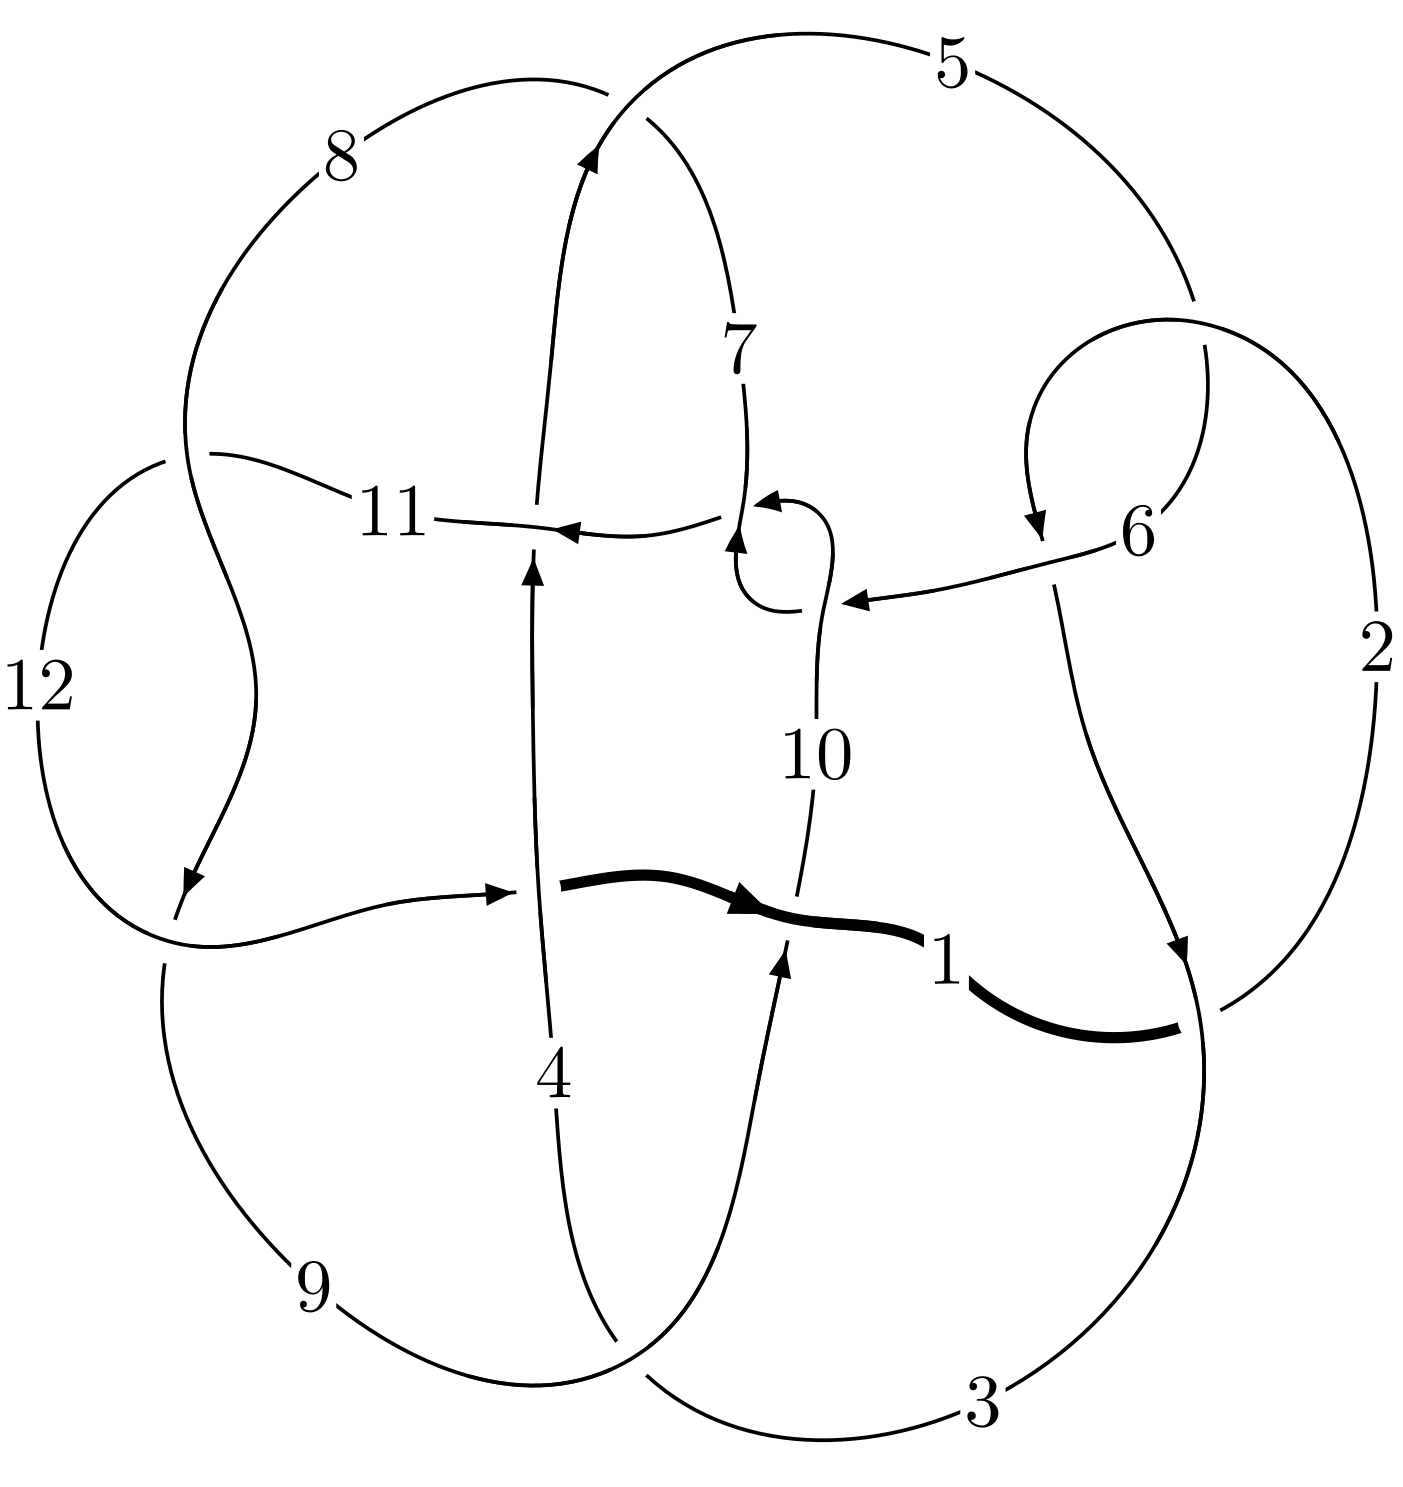
\includegraphics[width=112pt]{../../../GIT/diagram.site/Diagrams/png/1191_12a_0390.png}\\
\ \ \ A knot diagram\footnotemark}&
\allowdisplaybreaks
\textbf{Linearized knot diagam} \\
\cline{2-2}
 &
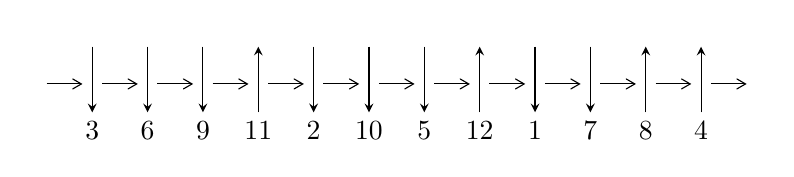
\begin{tikzpicture}[x=20pt, y=17pt]
	% nodes
	\node (C0) at (0, 0) {};
	\node (C1) at (1, 0) {};
	\node (C1U) at (1, +1) {};
	\node (C1D) at (1, -1) {3};

	\node (C2) at (2, 0) {};
	\node (C2U) at (2, +1) {};
	\node (C2D) at (2, -1) {6};

	\node (C3) at (3, 0) {};
	\node (C3U) at (3, +1) {};
	\node (C3D) at (3, -1) {9};

	\node (C4) at (4, 0) {};
	\node (C4U) at (4, +1) {};
	\node (C4D) at (4, -1) {11};

	\node (C5) at (5, 0) {};
	\node (C5U) at (5, +1) {};
	\node (C5D) at (5, -1) {2};

	\node (C6) at (6, 0) {};
	\node (C6U) at (6, +1) {};
	\node (C6D) at (6, -1) {10};

	\node (C7) at (7, 0) {};
	\node (C7U) at (7, +1) {};
	\node (C7D) at (7, -1) {5};

	\node (C8) at (8, 0) {};
	\node (C8U) at (8, +1) {};
	\node (C8D) at (8, -1) {12};

	\node (C9) at (9, 0) {};
	\node (C9U) at (9, +1) {};
	\node (C9D) at (9, -1) {1};

	\node (C10) at (10, 0) {};
	\node (C10U) at (10, +1) {};
	\node (C10D) at (10, -1) {7};

	\node (C11) at (11, 0) {};
	\node (C11U) at (11, +1) {};
	\node (C11D) at (11, -1) {8};

	\node (C12) at (12, 0) {};
	\node (C12U) at (12, +1) {};
	\node (C12D) at (12, -1) {4};
	\node (C13) at (13, 0) {};

	% arrows
	\draw[->,>={angle 60}]
	(C0) edge (C1) (C1) edge (C2) (C2) edge (C3) (C3) edge (C4) (C4) edge (C5) (C5) edge (C6) (C6) edge (C7) (C7) edge (C8) (C8) edge (C9) (C9) edge (C10) (C10) edge (C11) (C11) edge (C12) (C12) edge (C13) ;	\draw[->,>=stealth]
	(C1U) edge (C1D) (C2U) edge (C2D) (C3U) edge (C3D) (C4D) edge (C4U) (C5U) edge (C5D) (C6U) edge (C6D) (C7U) edge (C7D) (C8D) edge (C8U) (C9U) edge (C9D) (C10U) edge (C10D) (C11D) edge (C11U) (C12D) edge (C12U) ;
	\end{tikzpicture} \\
\hhline{~~} \\& 
\textbf{Solving Sequence} \\ \cline{2-2} 
 &
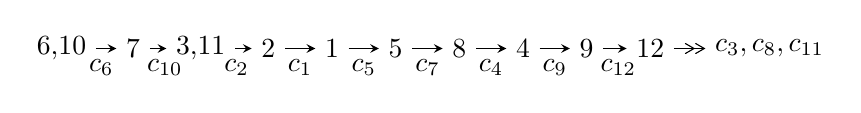
\begin{tikzpicture}[x=23pt, y=7pt]
	% node
	\node (A0) at (-1/8, 0) {6,10};
	\node (A1) at (1, 0) {7};
	\node (A2) at (33/16, 0) {3,11};
	\node (A3) at (25/8, 0) {2};
	\node (A4) at (33/8, 0) {1};
	\node (A5) at (41/8, 0) {5};
	\node (A6) at (49/8, 0) {8};
	\node (A7) at (57/8, 0) {4};
	\node (A8) at (65/8, 0) {9};
	\node (A9) at (73/8, 0) {12};
	\node (C1) at (1/2, -1) {$c_{6}$};
	\node (C2) at (3/2, -1) {$c_{10}$};
	\node (C3) at (21/8, -1) {$c_{2}$};
	\node (C4) at (29/8, -1) {$c_{1}$};
	\node (C5) at (37/8, -1) {$c_{5}$};
	\node (C6) at (45/8, -1) {$c_{7}$};
	\node (C7) at (53/8, -1) {$c_{4}$};
	\node (C8) at (61/8, -1) {$c_{9}$};
	\node (C9) at (69/8, -1) {$c_{12}$};
	\node (A10) at (11, 0) {$c_{3},c_{8},c_{11}$};

	% edge
	\draw[->,>=stealth]	
	(A0) edge (A1) (A1) edge (A2) (A2) edge (A3) (A3) edge (A4) (A4) edge (A5) (A5) edge (A6) (A6) edge (A7) (A7) edge (A8) (A8) edge (A9) ;
	\draw[->>,>={angle 60}]	
	(A9) edge (A10);
\end{tikzpicture} \\ 

\end{tabular} \\

\footnotetext{
The image of knot diagram is generated by the software ``\textbf{Draw programme}" developed by Andrew Bartholomew(\url{http://www.layer8.co.uk/maths/draw/index.htm\#Running-draw}), where we modified some parts for our purpose(\url{https://github.com/CATsTAILs/LinksPainter}).
}\phantom \\ \newline 
\centering \textbf{Ideals for irreducible components\footnotemark of $X_{\text{par}}$} 
 
\begin{align*}
I^u_{1}&=\langle 
5.37418\times10^{750} u^{144}-4.27866\times10^{751} u^{143}+\cdots+3.05104\times10^{751} b+1.85665\times10^{755},\\
\phantom{I^u_{1}}&\phantom{= \langle  }1.01579\times10^{754} u^{144}-8.04515\times10^{754} u^{143}+\cdots+3.45683\times10^{754} a+3.40763\times10^{758},\\
\phantom{I^u_{1}}&\phantom{= \langle  }u^{145}-9 u^{144}+\cdots+376000 u-36256\rangle \\
I^u_{2}&=\langle 
-1009040883105882 u^{27}-1315626392337378 u^{26}+\cdots+68752247482895 b-3458158094392594,\\
\phantom{I^u_{2}}&\phantom{= \langle  }-901563901956276 u^{27}-1137559180351494 u^{26}+\cdots+68752247482895 a-2992698774862172,\\
\phantom{I^u_{2}}&\phantom{= \langle  }u^{28}+u^{27}+\cdots+4 u-1\rangle \\
I^u_{3}&=\langle 
b+1,\;4 a^2+6 a- u+4,\;u^2-2\rangle \\
I^u_{4}&=\langle 
13787 a^8+73187 b+\cdots+77516 a+215532,\;a^9-5 a^7+23 a^5+20 a^4-12 a^3-10 a^2+19 a+11,\\
\phantom{I^u_{4}}&\phantom{= \langle  }u+1\rangle \\
\\
I^v_{1}&=\langle 
a,\;b+1,\;v-1\rangle \\
\end{align*}
\raggedright * 5 irreducible components of $\dim_{\mathbb{C}}=0$, with total 187 representations.\\
\footnotetext{All coefficients of polynomials are rational numbers. But the coefficients are sometimes approximated in decimal forms when there is not enough margin.}
\newpage
\renewcommand{\arraystretch}{1}
\centering \section*{I. $I^u_{1}= \langle 5.37\times10^{750} u^{144}-4.28\times10^{751} u^{143}+\cdots+3.05\times10^{751} b+1.86\times10^{755},\;1.02\times10^{754} u^{144}-8.05\times10^{754} u^{143}+\cdots+3.46\times10^{754} a+3.41\times10^{758},\;u^{145}-9 u^{144}+\cdots+376000 u-36256 \rangle$}
\flushleft \textbf{(i) Arc colorings}\\
\begin{tabular}{m{7pt} m{180pt} m{7pt} m{180pt} }
\flushright $a_{6}=$&$\begin{pmatrix}1\\0\end{pmatrix}$ \\
\flushright $a_{10}=$&$\begin{pmatrix}0\\u\end{pmatrix}$ \\
\flushright $a_{7}=$&$\begin{pmatrix}1\\u^2\end{pmatrix}$ \\
\flushright $a_{3}=$&$\begin{pmatrix}-0.293851 u^{144}+2.32732 u^{143}+\cdots+93139.9 u-9857.66\\-0.176142 u^{144}+1.40236 u^{143}+\cdots+57359.9 u-6085.29\end{pmatrix}$ \\
\flushright $a_{11}=$&$\begin{pmatrix}- u\\- u^3+u\end{pmatrix}$ \\
\flushright $a_{2}=$&$\begin{pmatrix}-0.469994 u^{144}+3.72968 u^{143}+\cdots+150500. u-15943.0\\-0.176142 u^{144}+1.40236 u^{143}+\cdots+57359.9 u-6085.29\end{pmatrix}$ \\
\flushright $a_{1}=$&$\begin{pmatrix}-0.0648032 u^{144}+0.499840 u^{143}+\cdots+17482.0 u-1820.92\\-0.536244 u^{144}+4.22100 u^{143}+\cdots+163169. u-17200.5\end{pmatrix}$ \\
\flushright $a_{5}=$&$\begin{pmatrix}-0.158282 u^{144}+1.27149 u^{143}+\cdots+54189.4 u-5772.13\\0.0630524 u^{144}-0.460147 u^{143}+\cdots-10118.6 u+963.721\end{pmatrix}$ \\
\flushright $a_{8}=$&$\begin{pmatrix}0.274941 u^{144}-2.19571 u^{143}+\cdots-91792.3 u+9764.90\\0.0105693 u^{144}-0.0829171 u^{143}+\cdots-3248.37 u+345.877\end{pmatrix}$ \\
\flushright $a_{4}=$&$\begin{pmatrix}-0.272586 u^{144}+2.14330 u^{143}+\cdots+81770.6 u-8595.38\\-0.0292223 u^{144}+0.263055 u^{143}+\cdots+17159.3 u-1902.46\end{pmatrix}$ \\
\flushright $a_{9}=$&$\begin{pmatrix}0.216468 u^{144}-1.69100 u^{143}+\cdots-61808.0 u+6459.95\\-0.0772742 u^{144}+0.598026 u^{143}+\cdots+21009.7 u-2186.39\end{pmatrix}$ \\
\flushright $a_{12}=$&$\begin{pmatrix}0.00595126 u^{144}-0.0196957 u^{143}+\cdots+5443.92 u-657.298\\-0.0957945 u^{144}+0.751906 u^{143}+\cdots+28689.4 u-3022.09\end{pmatrix}$\\&\end{tabular}
\flushleft \textbf{(ii) Obstruction class $= -1$}\\~\\
\flushleft \textbf{(iii) Cusp Shapes $= -2.18489 u^{144}+17.3876 u^{143}+\cdots+710362. u-75357.2$}\\~\\
\newpage\renewcommand{\arraystretch}{1}
\flushleft \textbf{(iv) u-Polynomials at the component}\newline \\
\begin{tabular}{m{50pt}|m{274pt}}
Crossings & \hspace{64pt}u-Polynomials at each crossing \\
\hline $$\begin{aligned}c_{1}\end{aligned}$$&$\begin{aligned}
&u^{145}+60 u^{144}+\cdots+69806531 u+3066001
\end{aligned}$\\
\hline $$\begin{aligned}c_{2},c_{5}\end{aligned}$$&$\begin{aligned}
&u^{145}-30 u^{143}+\cdots-5817 u+1751
\end{aligned}$\\
\hline $$\begin{aligned}c_{3}\end{aligned}$$&$\begin{aligned}
&2(2 u^{145}-2 u^{144}+\cdots-8207989 u+1252007)
\end{aligned}$\\
\hline $$\begin{aligned}c_{4}\end{aligned}$$&$\begin{aligned}
&2(2 u^{145}+6 u^{144}+\cdots-58 u-1)
\end{aligned}$\\
\hline $$\begin{aligned}c_{6},c_{10}\end{aligned}$$&$\begin{aligned}
&u^{145}-9 u^{144}+\cdots+376000 u-36256
\end{aligned}$\\
\hline $$\begin{aligned}c_{7}\end{aligned}$$&$\begin{aligned}
&u^{145}-10 u^{144}+\cdots-13808 u+958
\end{aligned}$\\
\hline $$\begin{aligned}c_{8},c_{11}\end{aligned}$$&$\begin{aligned}
&u^{145}- u^{144}+\cdots-402 u+9
\end{aligned}$\\
\hline $$\begin{aligned}c_{9}\end{aligned}$$&$\begin{aligned}
&u^{145}+7 u^{144}+\cdots-2484 u+124
\end{aligned}$\\
\hline $$\begin{aligned}c_{12}\end{aligned}$$&$\begin{aligned}
&u^{145}+14 u^{144}+\cdots+324 u+122
\end{aligned}$\\
\hline
\end{tabular}\\~\\
\newpage\renewcommand{\arraystretch}{1}
\flushleft \textbf{(v) Riley Polynomials at the component}\newline \\
\begin{tabular}{m{50pt}|m{274pt}}
Crossings & \hspace{64pt}Riley Polynomials at each crossing \\
\hline $$\begin{aligned}c_{1}\end{aligned}$$&$\begin{aligned}
&y^{145}+52 y^{144}+\cdots-76219022336469 y-9400362132001
\end{aligned}$\\
\hline $$\begin{aligned}c_{2},c_{5}\end{aligned}$$&$\begin{aligned}
&y^{145}-60 y^{144}+\cdots+69806531 y-3066001
\end{aligned}$\\
\hline $$\begin{aligned}c_{3}\end{aligned}$$&$\begin{aligned}
&4(4 y^{145}+224 y^{144}+\cdots-3.85023\times10^{13} y-1.56752\times10^{12})
\end{aligned}$\\
\hline $$\begin{aligned}c_{4}\end{aligned}$$&$\begin{aligned}
&4(4 y^{145}+80 y^{144}+\cdots+1062 y-1)
\end{aligned}$\\
\hline $$\begin{aligned}c_{6},c_{10}\end{aligned}$$&$\begin{aligned}
&y^{145}-99 y^{144}+\cdots-18148659712 y-1314497536
\end{aligned}$\\
\hline $$\begin{aligned}c_{7}\end{aligned}$$&$\begin{aligned}
&y^{145}+24 y^{144}+\cdots-104405052 y-917764
\end{aligned}$\\
\hline $$\begin{aligned}c_{8},c_{11}\end{aligned}$$&$\begin{aligned}
&y^{145}-111 y^{144}+\cdots+29430 y-81
\end{aligned}$\\
\hline $$\begin{aligned}c_{9}\end{aligned}$$&$\begin{aligned}
&y^{145}-17 y^{144}+\cdots+17645216 y-15376
\end{aligned}$\\
\hline $$\begin{aligned}c_{12}\end{aligned}$$&$\begin{aligned}
&y^{145}-2 y^{144}+\cdots-585788 y-14884
\end{aligned}$\\
\hline
\end{tabular}\\~\\
\newpage\flushleft \textbf{(vi) Complex Volumes and Cusp Shapes}
$$\begin{array}{c|c|c}  
\text{Solutions to }I^u_{1}& \I (\text{vol} + \sqrt{-1}CS) & \text{Cusp shape}\\
 \hline 
\begin{aligned}
u &= \phantom{-}0.983060 + 0.090094 I \\
a &= \phantom{-}2.13665 + 1.88345 I \\
b &= \phantom{-}0.858935 - 0.384607 I\end{aligned}
 & \phantom{-}1.62861 - 5.53148 I & \phantom{-0.000000 } 0 \\ \hline\begin{aligned}
u &= \phantom{-}0.983060 - 0.090094 I \\
a &= \phantom{-}2.13665 - 1.88345 I \\
b &= \phantom{-}0.858935 + 0.384607 I\end{aligned}
 & \phantom{-}1.62861 + 5.53148 I & \phantom{-0.000000 } 0 \\ \hline\begin{aligned}
u &= -0.685449 + 0.758061 I \\
a &= \phantom{-}0.427863 + 1.187920 I \\
b &= \phantom{-}0.598913 - 0.804263 I\end{aligned}
 & \phantom{-}5.68349 + 0.09462 I & \phantom{-0.000000 } 0 \\ \hline\begin{aligned}
u &= -0.685449 - 0.758061 I \\
a &= \phantom{-}0.427863 - 1.187920 I \\
b &= \phantom{-}0.598913 + 0.804263 I\end{aligned}
 & \phantom{-}5.68349 - 0.09462 I & \phantom{-0.000000 } 0 \\ \hline\begin{aligned}
u &= \phantom{-}0.254251 + 0.937529 I \\
a &= \phantom{-}0.89791 + 1.30032 I \\
b &= -0.888302 - 0.707889 I\end{aligned}
 & \phantom{-}6.32851 + 0.10858 I & \phantom{-0.000000 } 0 \\ \hline\begin{aligned}
u &= \phantom{-}0.254251 - 0.937529 I \\
a &= \phantom{-}0.89791 - 1.30032 I \\
b &= -0.888302 + 0.707889 I\end{aligned}
 & \phantom{-}6.32851 - 0.10858 I & \phantom{-0.000000 } 0 \\ \hline\begin{aligned}
u &= \phantom{-}0.713038 + 0.747574 I \\
a &= -0.790441 + 0.231774 I \\
b &= \phantom{-}0.857271 + 0.045849 I\end{aligned}
 & \phantom{-}1.34056 - 7.92861 I & \phantom{-0.000000 } 0 \\ \hline\begin{aligned}
u &= \phantom{-}0.713038 - 0.747574 I \\
a &= -0.790441 - 0.231774 I \\
b &= \phantom{-}0.857271 - 0.045849 I\end{aligned}
 & \phantom{-}1.34056 + 7.92861 I & \phantom{-0.000000 } 0 \\ \hline\begin{aligned}
u &= \phantom{-}0.811575 + 0.514492 I \\
a &= \phantom{-}0.53915 + 1.35311 I \\
b &= \phantom{-}0.605411 - 0.223383 I\end{aligned}
 & \phantom{-}1.75716 + 3.74479 I & \phantom{-0.000000 } 0 \\ \hline\begin{aligned}
u &= \phantom{-}0.811575 - 0.514492 I \\
a &= \phantom{-}0.53915 - 1.35311 I \\
b &= \phantom{-}0.605411 + 0.223383 I\end{aligned}
 & \phantom{-}1.75716 - 3.74479 I & \phantom{-0.000000 } 0\\
 \hline 
 \end{array}$$\newpage$$\begin{array}{c|c|c}  
\text{Solutions to }I^u_{1}& \I (\text{vol} + \sqrt{-1}CS) & \text{Cusp shape}\\
 \hline 
\begin{aligned}
u &= \phantom{-}0.897025 + 0.529202 I \\
a &= -0.331859 - 0.105549 I \\
b &= \phantom{-}0.735731 - 0.625405 I\end{aligned}
 & \phantom{-}4.30487 + 1.12753 I & \phantom{-0.000000 } 0 \\ \hline\begin{aligned}
u &= \phantom{-}0.897025 - 0.529202 I \\
a &= -0.331859 + 0.105549 I \\
b &= \phantom{-}0.735731 + 0.625405 I\end{aligned}
 & \phantom{-}4.30487 - 1.12753 I & \phantom{-0.000000 } 0 \\ \hline\begin{aligned}
u &= -0.517746 + 0.906672 I \\
a &= -0.545481 - 0.539143 I \\
b &= \phantom{-}1.038390 + 0.664944 I\end{aligned}
 & \phantom{-}4.34586 - 5.42296 I & \phantom{-0.000000 } 0 \\ \hline\begin{aligned}
u &= -0.517746 - 0.906672 I \\
a &= -0.545481 + 0.539143 I \\
b &= \phantom{-}1.038390 - 0.664944 I\end{aligned}
 & \phantom{-}4.34586 + 5.42296 I & \phantom{-0.000000 } 0 \\ \hline\begin{aligned}
u &= -1.050360 + 0.161995 I \\
a &= \phantom{-}0.51067 + 2.23058 I \\
b &= \phantom{-}1.040340 - 0.654724 I\end{aligned}
 & -2.96212 + 5.40060 I & \phantom{-0.000000 } 0 \\ \hline\begin{aligned}
u &= -1.050360 - 0.161995 I \\
a &= \phantom{-}0.51067 - 2.23058 I \\
b &= \phantom{-}1.040340 + 0.654724 I\end{aligned}
 & -2.96212 - 5.40060 I & \phantom{-0.000000 } 0 \\ \hline\begin{aligned}
u &= -0.805102 + 0.476131 I \\
a &= -0.598161 - 0.563764 I \\
b &= \phantom{-}0.356213 + 1.008710 I\end{aligned}
 & \phantom{-}5.20952 + 4.67407 I & \phantom{-0.000000 } 0 \\ \hline\begin{aligned}
u &= -0.805102 - 0.476131 I \\
a &= -0.598161 + 0.563764 I \\
b &= \phantom{-}0.356213 - 1.008710 I\end{aligned}
 & \phantom{-}5.20952 - 4.67407 I & \phantom{-0.000000 } 0 \\ \hline\begin{aligned}
u &= -0.882698 + 0.612745 I \\
a &= \phantom{-}1.071400 + 0.504659 I \\
b &= -0.768499 - 0.480559 I\end{aligned}
 & -0.650607 + 0.239775 I & \phantom{-0.000000 } 0 \\ \hline\begin{aligned}
u &= -0.882698 - 0.612745 I \\
a &= \phantom{-}1.071400 - 0.504659 I \\
b &= -0.768499 + 0.480559 I\end{aligned}
 & -0.650607 - 0.239775 I & \phantom{-0.000000 } 0\\
 \hline 
 \end{array}$$\newpage$$\begin{array}{c|c|c}  
\text{Solutions to }I^u_{1}& \I (\text{vol} + \sqrt{-1}CS) & \text{Cusp shape}\\
 \hline 
\begin{aligned}
u &= -1.072310 + 0.173522 I \\
a &= \phantom{-}0.034423 - 0.580747 I \\
b &= -0.425481 + 1.312410 I\end{aligned}
 & \phantom{-}2.71130 + 6.68388 I & \phantom{-0.000000 } 0 \\ \hline\begin{aligned}
u &= -1.072310 - 0.173522 I \\
a &= \phantom{-}0.034423 + 0.580747 I \\
b &= -0.425481 - 1.312410 I\end{aligned}
 & \phantom{-}2.71130 - 6.68388 I & \phantom{-0.000000 } 0 \\ \hline\begin{aligned}
u &= \phantom{-}1.082880 + 0.160074 I \\
a &= \phantom{-}0.188167 + 0.739468 I \\
b &= -0.499543 - 0.904517 I\end{aligned}
 & -2.70646 - 3.57717 I & \phantom{-0.000000 } 0 \\ \hline\begin{aligned}
u &= \phantom{-}1.082880 - 0.160074 I \\
a &= \phantom{-}0.188167 - 0.739468 I \\
b &= -0.499543 + 0.904517 I\end{aligned}
 & -2.70646 + 3.57717 I & \phantom{-0.000000 } 0 \\ \hline\begin{aligned}
u &= \phantom{-}0.891059 + 0.068423 I \\
a &= -0.285409 - 1.230440 I \\
b &= \phantom{-}0.924124 + 0.930627 I\end{aligned}
 & \phantom{-}5.54059 - 3.39336 I & \phantom{-0.000000 } 0 \\ \hline\begin{aligned}
u &= \phantom{-}0.891059 - 0.068423 I \\
a &= -0.285409 + 1.230440 I \\
b &= \phantom{-}0.924124 - 0.930627 I\end{aligned}
 & \phantom{-}5.54059 + 3.39336 I & \phantom{-0.000000 } 0 \\ \hline\begin{aligned}
u &= \phantom{-}0.222169 + 0.852674 I \\
a &= -0.642834 + 0.938742 I \\
b &= \phantom{-}1.010100 - 0.613224 I\end{aligned}
 & \phantom{-}1.75366 + 4.60471 I & \phantom{-0.000000 } 0 \\ \hline\begin{aligned}
u &= \phantom{-}0.222169 - 0.852674 I \\
a &= -0.642834 - 0.938742 I \\
b &= \phantom{-}1.010100 + 0.613224 I\end{aligned}
 & \phantom{-}1.75366 - 4.60471 I & \phantom{-0.000000 } 0 \\ \hline\begin{aligned}
u &= \phantom{-}1.091750 + 0.259485 I \\
a &= \phantom{-}1.028000 - 0.914616 I \\
b &= \phantom{-}0.914032 + 0.618678 I\end{aligned}
 & \phantom{-}3.76788 - 3.76551 I & \phantom{-0.000000 } 0 \\ \hline\begin{aligned}
u &= \phantom{-}1.091750 - 0.259485 I \\
a &= \phantom{-}1.028000 + 0.914616 I \\
b &= \phantom{-}0.914032 - 0.618678 I\end{aligned}
 & \phantom{-}3.76788 + 3.76551 I & \phantom{-0.000000 } 0\\
 \hline 
 \end{array}$$\newpage$$\begin{array}{c|c|c}  
\text{Solutions to }I^u_{1}& \I (\text{vol} + \sqrt{-1}CS) & \text{Cusp shape}\\
 \hline 
\begin{aligned}
u &= \phantom{-}0.388134 + 0.782870 I \\
a &= \phantom{-}0.386454 - 0.846415 I \\
b &= \phantom{-}0.174351 + 0.409736 I\end{aligned}
 & \phantom{-}2.48869 + 1.37898 I & \phantom{-0.000000 } 0 \\ \hline\begin{aligned}
u &= \phantom{-}0.388134 - 0.782870 I \\
a &= \phantom{-}0.386454 + 0.846415 I \\
b &= \phantom{-}0.174351 - 0.409736 I\end{aligned}
 & \phantom{-}2.48869 - 1.37898 I & \phantom{-0.000000 } 0 \\ \hline\begin{aligned}
u &= \phantom{-}1.122820 + 0.087405 I \\
a &= -0.609964 + 1.068290 I \\
b &= -1.187300 - 0.657079 I\end{aligned}
 & -4.77701 - 2.45139 I & \phantom{-0.000000 } 0 \\ \hline\begin{aligned}
u &= \phantom{-}1.122820 - 0.087405 I \\
a &= -0.609964 - 1.068290 I \\
b &= -1.187300 + 0.657079 I\end{aligned}
 & -4.77701 + 2.45139 I & \phantom{-0.000000 } 0 \\ \hline\begin{aligned}
u &= \phantom{-}1.065620 + 0.364968 I \\
a &= -0.485814 + 0.394476 I \\
b &= \phantom{-}0.367234 - 0.928765 I\end{aligned}
 & \phantom{-}0.92008 - 3.52870 I & \phantom{-0.000000 } 0 \\ \hline\begin{aligned}
u &= \phantom{-}1.065620 - 0.364968 I \\
a &= -0.485814 - 0.394476 I \\
b &= \phantom{-}0.367234 + 0.928765 I\end{aligned}
 & \phantom{-}0.92008 + 3.52870 I & \phantom{-0.000000 } 0 \\ \hline\begin{aligned}
u &= -0.020658 + 1.128840 I \\
a &= \phantom{-}0.14589 - 1.41304 I \\
b &= -0.614229 + 0.797164 I\end{aligned}
 & \phantom{-}7.05249 - 7.91380 I & \phantom{-0.000000 } 0 \\ \hline\begin{aligned}
u &= -0.020658 - 1.128840 I \\
a &= \phantom{-}0.14589 + 1.41304 I \\
b &= -0.614229 - 0.797164 I\end{aligned}
 & \phantom{-}7.05249 + 7.91380 I & \phantom{-0.000000 } 0 \\ \hline\begin{aligned}
u &= -0.745702 + 0.850929 I \\
a &= -0.204447 - 0.338471 I \\
b &= \phantom{-}0.784925 + 0.090674 I\end{aligned}
 & -2.54065 + 2.41226 I & \phantom{-0.000000 } 0 \\ \hline\begin{aligned}
u &= -0.745702 - 0.850929 I \\
a &= -0.204447 + 0.338471 I \\
b &= \phantom{-}0.784925 - 0.090674 I\end{aligned}
 & -2.54065 - 2.41226 I & \phantom{-0.000000 } 0\\
 \hline 
 \end{array}$$\newpage$$\begin{array}{c|c|c}  
\text{Solutions to }I^u_{1}& \I (\text{vol} + \sqrt{-1}CS) & \text{Cusp shape}\\
 \hline 
\begin{aligned}
u &= \phantom{-}1.140260 + 0.090079 I \\
a &= -0.760401 + 0.140342 I \\
b &= \phantom{-}0.370111 - 0.802407 I\end{aligned}
 & \phantom{-}0.41878 - 4.86981 I & \phantom{-0.000000 } 0 \\ \hline\begin{aligned}
u &= \phantom{-}1.140260 - 0.090079 I \\
a &= -0.760401 - 0.140342 I \\
b &= \phantom{-}0.370111 + 0.802407 I\end{aligned}
 & \phantom{-}0.41878 + 4.86981 I & \phantom{-0.000000 } 0 \\ \hline\begin{aligned}
u &= -1.16430\phantom{ +0.000000I} \\
a &= -0.916535\phantom{ +0.000000I} \\
b &= -1.55885\phantom{ +0.000000I}\end{aligned}
 & -2.35115\phantom{ +0.000000I} & \phantom{-0.000000 } 0 \\ \hline\begin{aligned}
u &= \phantom{-}0.151303 + 0.819847 I \\
a &= -0.33031 - 1.37740 I \\
b &= \phantom{-}1.005360 + 0.727730 I\end{aligned}
 & \phantom{-}6.54392 - 5.53486 I & \phantom{-0.000000 } 0 \\ \hline\begin{aligned}
u &= \phantom{-}0.151303 - 0.819847 I \\
a &= -0.33031 + 1.37740 I \\
b &= \phantom{-}1.005360 - 0.727730 I\end{aligned}
 & \phantom{-}6.54392 + 5.53486 I & \phantom{-0.000000 } 0 \\ \hline\begin{aligned}
u &= -1.041960 + 0.548317 I \\
a &= \phantom{-}0.53446 + 1.47256 I \\
b &= \phantom{-}1.199300 - 0.678298 I\end{aligned}
 & \phantom{-}2.66277 + 10.75610 I & \phantom{-0.000000 } 0 \\ \hline\begin{aligned}
u &= -1.041960 - 0.548317 I \\
a &= \phantom{-}0.53446 - 1.47256 I \\
b &= \phantom{-}1.199300 + 0.678298 I\end{aligned}
 & \phantom{-}2.66277 - 10.75610 I & \phantom{-0.000000 } 0 \\ \hline\begin{aligned}
u &= -1.144180 + 0.280710 I \\
a &= -0.52536 - 1.89176 I \\
b &= -1.010730 + 0.507563 I\end{aligned}
 & -3.26054 + 4.10580 I & \phantom{-0.000000 } 0 \\ \hline\begin{aligned}
u &= -1.144180 - 0.280710 I \\
a &= -0.52536 + 1.89176 I \\
b &= -1.010730 - 0.507563 I\end{aligned}
 & -3.26054 - 4.10580 I & \phantom{-0.000000 } 0 \\ \hline\begin{aligned}
u &= \phantom{-}1.18550\phantom{ +0.000000I} \\
a &= -0.763855\phantom{ +0.000000I} \\
b &= -1.37910\phantom{ +0.000000I}\end{aligned}
 & -5.52230\phantom{ +0.000000I} & \phantom{-0.000000 } 0\\
 \hline 
 \end{array}$$\newpage$$\begin{array}{c|c|c}  
\text{Solutions to }I^u_{1}& \I (\text{vol} + \sqrt{-1}CS) & \text{Cusp shape}\\
 \hline 
\begin{aligned}
u &= \phantom{-}1.195690 + 0.166098 I \\
a &= \phantom{-}0.07704 + 1.68510 I \\
b &= -0.885702 - 0.531747 I\end{aligned}
 & -3.13450 - 2.17134 I & \phantom{-0.000000 } 0 \\ \hline\begin{aligned}
u &= \phantom{-}1.195690 - 0.166098 I \\
a &= \phantom{-}0.07704 - 1.68510 I \\
b &= -0.885702 + 0.531747 I\end{aligned}
 & -3.13450 + 2.17134 I & \phantom{-0.000000 } 0 \\ \hline\begin{aligned}
u &= \phantom{-}0.147231 + 0.776960 I \\
a &= \phantom{-}0.04260 - 2.01983 I \\
b &= -0.837232 + 0.751778 I\end{aligned}
 & \phantom{-}6.51195 + 5.65463 I & \phantom{-0.000000 } 0 \\ \hline\begin{aligned}
u &= \phantom{-}0.147231 - 0.776960 I \\
a &= \phantom{-}0.04260 + 2.01983 I \\
b &= -0.837232 - 0.751778 I\end{aligned}
 & \phantom{-}6.51195 - 5.65463 I & \phantom{-0.000000 } 0 \\ \hline\begin{aligned}
u &= \phantom{-}0.401631 + 0.679622 I \\
a &= \phantom{-}0.10653 - 1.43292 I \\
b &= \phantom{-}0.607703 + 0.710606 I\end{aligned}
 & \phantom{-}2.97272 - 0.48461 I & \phantom{-0.000000 } 0 \\ \hline\begin{aligned}
u &= \phantom{-}0.401631 - 0.679622 I \\
a &= \phantom{-}0.10653 + 1.43292 I \\
b &= \phantom{-}0.607703 - 0.710606 I\end{aligned}
 & \phantom{-}2.97272 + 0.48461 I & \phantom{-0.000000 } 0 \\ \hline\begin{aligned}
u &= \phantom{-}1.191400 + 0.220075 I \\
a &= \phantom{-}1.02025 - 1.77251 I \\
b &= \phantom{-}1.126050 + 0.612022 I\end{aligned}
 & -1.78712 - 10.16790 I & \phantom{-0.000000 } 0 \\ \hline\begin{aligned}
u &= \phantom{-}1.191400 - 0.220075 I \\
a &= \phantom{-}1.02025 + 1.77251 I \\
b &= \phantom{-}1.126050 - 0.612022 I\end{aligned}
 & -1.78712 + 10.16790 I & \phantom{-0.000000 } 0 \\ \hline\begin{aligned}
u &= -0.072552 + 0.782684 I \\
a &= -0.349628 + 1.314310 I \\
b &= \phantom{-}0.668772 - 0.847851 I\end{aligned}
 & \phantom{-}7.56826 + 0.30824 I & \phantom{-0.000000 } 0 \\ \hline\begin{aligned}
u &= -0.072552 - 0.782684 I \\
a &= -0.349628 - 1.314310 I \\
b &= \phantom{-}0.668772 + 0.847851 I\end{aligned}
 & \phantom{-}7.56826 - 0.30824 I & \phantom{-0.000000 } 0\\
 \hline 
 \end{array}$$\newpage$$\begin{array}{c|c|c}  
\text{Solutions to }I^u_{1}& \I (\text{vol} + \sqrt{-1}CS) & \text{Cusp shape}\\
 \hline 
\begin{aligned}
u &= -1.128570 + 0.485023 I \\
a &= -1.04988 - 1.87414 I \\
b &= -0.910652 + 0.519441 I\end{aligned}
 & -1.11152 + 4.37732 I & \phantom{-0.000000 } 0 \\ \hline\begin{aligned}
u &= -1.128570 - 0.485023 I \\
a &= -1.04988 + 1.87414 I \\
b &= -0.910652 - 0.519441 I\end{aligned}
 & -1.11152 - 4.37732 I & \phantom{-0.000000 } 0 \\ \hline\begin{aligned}
u &= \phantom{-}0.095858 + 1.241060 I \\
a &= \phantom{-}0.22271 + 1.49312 I \\
b &= -0.674538 - 0.650534 I\end{aligned}
 & \phantom{-}1.47619 + 2.13178 I & \phantom{-0.000000 } 0 \\ \hline\begin{aligned}
u &= \phantom{-}0.095858 - 1.241060 I \\
a &= \phantom{-}0.22271 - 1.49312 I \\
b &= -0.674538 + 0.650534 I\end{aligned}
 & \phantom{-}1.47619 - 2.13178 I & \phantom{-0.000000 } 0 \\ \hline\begin{aligned}
u &= \phantom{-}0.197748 + 1.255820 I \\
a &= -0.268541 + 0.928652 I \\
b &= \phantom{-}0.954939 - 0.502519 I\end{aligned}
 & \phantom{-}0.95875 + 4.85612 I & \phantom{-0.000000 } 0 \\ \hline\begin{aligned}
u &= \phantom{-}0.197748 - 1.255820 I \\
a &= -0.268541 - 0.928652 I \\
b &= \phantom{-}0.954939 + 0.502519 I\end{aligned}
 & \phantom{-}0.95875 - 4.85612 I & \phantom{-0.000000 } 0 \\ \hline\begin{aligned}
u &= -1.213160 + 0.408995 I \\
a &= -0.360762 - 0.243484 I \\
b &= \phantom{-}0.400987 + 0.946443 I\end{aligned}
 & \phantom{-}4.07967 + 4.04266 I & \phantom{-0.000000 } 0 \\ \hline\begin{aligned}
u &= -1.213160 - 0.408995 I \\
a &= -0.360762 + 0.243484 I \\
b &= \phantom{-}0.400987 - 0.946443 I\end{aligned}
 & \phantom{-}4.07967 - 4.04266 I & \phantom{-0.000000 } 0 \\ \hline\begin{aligned}
u &= \phantom{-}1.223850 + 0.423966 I \\
a &= \phantom{-}0.72684 - 1.43560 I \\
b &= \phantom{-}1.159680 + 0.644217 I\end{aligned}
 & -1.45588 - 9.25214 I & \phantom{-0.000000 } 0 \\ \hline\begin{aligned}
u &= \phantom{-}1.223850 - 0.423966 I \\
a &= \phantom{-}0.72684 + 1.43560 I \\
b &= \phantom{-}1.159680 - 0.644217 I\end{aligned}
 & -1.45588 + 9.25214 I & \phantom{-0.000000 } 0\\
 \hline 
 \end{array}$$\newpage$$\begin{array}{c|c|c}  
\text{Solutions to }I^u_{1}& \I (\text{vol} + \sqrt{-1}CS) & \text{Cusp shape}\\
 \hline 
\begin{aligned}
u &= -0.667302 + 0.203508 I \\
a &= -1.36130 + 1.03136 I \\
b &= \phantom{-}0.909212 + 0.467787 I\end{aligned}
 & -1.81635 - 3.73460 I & \phantom{-0.000000 } 0 \\ \hline\begin{aligned}
u &= -0.667302 - 0.203508 I \\
a &= -1.36130 - 1.03136 I \\
b &= \phantom{-}0.909212 - 0.467787 I\end{aligned}
 & -1.81635 + 3.73460 I & \phantom{-0.000000 } 0 \\ \hline\begin{aligned}
u &= \phantom{-}0.134120 + 1.295810 I \\
a &= \phantom{-}0.426303 + 1.227870 I \\
b &= -1.033780 - 0.669869 I\end{aligned}
 & \phantom{-}5.7731 - 13.4390 I & \phantom{-0.000000 } 0 \\ \hline\begin{aligned}
u &= \phantom{-}0.134120 - 1.295810 I \\
a &= \phantom{-}0.426303 - 1.227870 I \\
b &= -1.033780 + 0.669869 I\end{aligned}
 & \phantom{-}5.7731 + 13.4390 I & \phantom{-0.000000 } 0 \\ \hline\begin{aligned}
u &= \phantom{-}1.263880 + 0.347113 I \\
a &= -0.435669 - 0.253457 I \\
b &= -1.271320 + 0.282733 I\end{aligned}
 & -4.64492 - 2.87820 I & \phantom{-0.000000 } 0 \\ \hline\begin{aligned}
u &= \phantom{-}1.263880 - 0.347113 I \\
a &= -0.435669 + 0.253457 I \\
b &= -1.271320 - 0.282733 I\end{aligned}
 & -4.64492 + 2.87820 I & \phantom{-0.000000 } 0 \\ \hline\begin{aligned}
u &= \phantom{-}1.196060 + 0.552992 I \\
a &= \phantom{-}0.748770 + 0.074311 I \\
b &= -0.754108 + 0.572872 I\end{aligned}
 & \phantom{-}3.40962 - 5.46166 I & \phantom{-0.000000 } 0 \\ \hline\begin{aligned}
u &= \phantom{-}1.196060 - 0.552992 I \\
a &= \phantom{-}0.748770 - 0.074311 I \\
b &= -0.754108 - 0.572872 I\end{aligned}
 & \phantom{-}3.40962 + 5.46166 I & \phantom{-0.000000 } 0 \\ \hline\begin{aligned}
u &= -0.163988 + 0.661489 I \\
a &= \phantom{-}1.64018 + 1.79230 I \\
b &= -0.962143 - 0.280015 I\end{aligned}
 & -0.361799 - 0.690892 I & \phantom{-0.000000 } 0 \\ \hline\begin{aligned}
u &= -0.163988 - 0.661489 I \\
a &= \phantom{-}1.64018 - 1.79230 I \\
b &= -0.962143 + 0.280015 I\end{aligned}
 & -0.361799 + 0.690892 I & \phantom{-0.000000 } 0\\
 \hline 
 \end{array}$$\newpage$$\begin{array}{c|c|c}  
\text{Solutions to }I^u_{1}& \I (\text{vol} + \sqrt{-1}CS) & \text{Cusp shape}\\
 \hline 
\begin{aligned}
u &= -1.113060 + 0.715277 I \\
a &= \phantom{-}0.739715 + 1.048430 I \\
b &= -0.673595 - 0.730560 I\end{aligned}
 & -0.344412 + 1.034890 I & \phantom{-0.000000 } 0 \\ \hline\begin{aligned}
u &= -1.113060 - 0.715277 I \\
a &= \phantom{-}0.739715 - 1.048430 I \\
b &= -0.673595 + 0.730560 I\end{aligned}
 & -0.344412 - 1.034890 I & \phantom{-0.000000 } 0 \\ \hline\begin{aligned}
u &= \phantom{-}1.322570 + 0.039753 I \\
a &= -1.117680 + 0.298273 I \\
b &= -1.233860 + 0.200738 I\end{aligned}
 & -4.69333 - 1.90088 I & \phantom{-0.000000 } 0 \\ \hline\begin{aligned}
u &= \phantom{-}1.322570 - 0.039753 I \\
a &= -1.117680 - 0.298273 I \\
b &= -1.233860 - 0.200738 I\end{aligned}
 & -4.69333 + 1.90088 I & \phantom{-0.000000 } 0 \\ \hline\begin{aligned}
u &= \phantom{-}1.202510 + 0.570331 I \\
a &= -0.353545 + 0.664942 I \\
b &= \phantom{-}0.189724 - 0.795449 I\end{aligned}
 & -0.02933 - 6.64809 I & \phantom{-0.000000 } 0 \\ \hline\begin{aligned}
u &= \phantom{-}1.202510 - 0.570331 I \\
a &= -0.353545 - 0.664942 I \\
b &= \phantom{-}0.189724 + 0.795449 I\end{aligned}
 & -0.02933 + 6.64809 I & \phantom{-0.000000 } 0 \\ \hline\begin{aligned}
u &= \phantom{-}1.286650 + 0.403088 I \\
a &= -1.41755 + 1.36786 I \\
b &= -0.927742 - 0.564801 I\end{aligned}
 & \phantom{-}2.85902 - 10.00570 I & \phantom{-0.000000 } 0 \\ \hline\begin{aligned}
u &= \phantom{-}1.286650 - 0.403088 I \\
a &= -1.41755 - 1.36786 I \\
b &= -0.927742 + 0.564801 I\end{aligned}
 & \phantom{-}2.85902 + 10.00570 I & \phantom{-0.000000 } 0 \\ \hline\begin{aligned}
u &= -1.354830 + 0.043354 I \\
a &= -1.020840 - 0.838053 I \\
b &= -0.971571 - 0.166745 I\end{aligned}
 & -6.45997 - 0.55941 I & \phantom{-0.000000 } 0 \\ \hline\begin{aligned}
u &= -1.354830 - 0.043354 I \\
a &= -1.020840 + 0.838053 I \\
b &= -0.971571 + 0.166745 I\end{aligned}
 & -6.45997 + 0.55941 I & \phantom{-0.000000 } 0\\
 \hline 
 \end{array}$$\newpage$$\begin{array}{c|c|c}  
\text{Solutions to }I^u_{1}& \I (\text{vol} + \sqrt{-1}CS) & \text{Cusp shape}\\
 \hline 
\begin{aligned}
u &= -1.349680 + 0.132285 I \\
a &= -0.208976 - 0.975259 I \\
b &= -1.060970 + 0.900995 I\end{aligned}
 & \phantom{-}0.48168 + 3.59119 I & \phantom{-0.000000 } 0 \\ \hline\begin{aligned}
u &= -1.349680 - 0.132285 I \\
a &= -0.208976 + 0.975259 I \\
b &= -1.060970 - 0.900995 I\end{aligned}
 & \phantom{-}0.48168 - 3.59119 I & \phantom{-0.000000 } 0 \\ \hline\begin{aligned}
u &= -1.254560 + 0.522994 I \\
a &= -0.213295 - 0.748929 I \\
b &= \phantom{-}0.339254 + 0.625085 I\end{aligned}
 & -3.15308 + 1.99288 I & \phantom{-0.000000 } 0 \\ \hline\begin{aligned}
u &= -1.254560 - 0.522994 I \\
a &= -0.213295 + 0.748929 I \\
b &= \phantom{-}0.339254 - 0.625085 I\end{aligned}
 & -3.15308 - 1.99288 I & \phantom{-0.000000 } 0 \\ \hline\begin{aligned}
u &= -1.339420 + 0.290116 I \\
a &= \phantom{-}0.611052 + 0.186561 I \\
b &= \phantom{-}1.365420 - 0.069213 I\end{aligned}
 & -4.43721 + 10.90670 I & \phantom{-0.000000 } 0 \\ \hline\begin{aligned}
u &= -1.339420 - 0.290116 I \\
a &= \phantom{-}0.611052 - 0.186561 I \\
b &= \phantom{-}1.365420 + 0.069213 I\end{aligned}
 & -4.43721 - 10.90670 I & \phantom{-0.000000 } 0 \\ \hline\begin{aligned}
u &= -1.36887 + 0.38491 I \\
a &= \phantom{-}0.86717 + 1.19426 I \\
b &= \phantom{-}1.163830 - 0.669799 I\end{aligned}
 & \phantom{-}1.77972 + 9.93298 I & \phantom{-0.000000 } 0 \\ \hline\begin{aligned}
u &= -1.36887 - 0.38491 I \\
a &= \phantom{-}0.86717 - 1.19426 I \\
b &= \phantom{-}1.163830 + 0.669799 I\end{aligned}
 & \phantom{-}1.77972 - 9.93298 I & \phantom{-0.000000 } 0 \\ \hline\begin{aligned}
u &= \phantom{-}1.39704 + 0.27963 I \\
a &= \phantom{-}0.627760 - 0.164251 I \\
b &= \phantom{-}1.239420 + 0.027842 I\end{aligned}
 & -9.04489 - 6.00167 I & \phantom{-0.000000 } 0 \\ \hline\begin{aligned}
u &= \phantom{-}1.39704 - 0.27963 I \\
a &= \phantom{-}0.627760 + 0.164251 I \\
b &= \phantom{-}1.239420 - 0.027842 I\end{aligned}
 & -9.04489 + 6.00167 I & \phantom{-0.000000 } 0\\
 \hline 
 \end{array}$$\newpage$$\begin{array}{c|c|c}  
\text{Solutions to }I^u_{1}& \I (\text{vol} + \sqrt{-1}CS) & \text{Cusp shape}\\
 \hline 
\begin{aligned}
u &= \phantom{-}1.32420 + 0.54500 I \\
a &= \phantom{-}0.549841 - 0.699856 I \\
b &= -0.521281 + 0.903568 I\end{aligned}
 & -2.43041 - 8.09154 I & \phantom{-0.000000 } 0 \\ \hline\begin{aligned}
u &= \phantom{-}1.32420 - 0.54500 I \\
a &= \phantom{-}0.549841 + 0.699856 I \\
b &= -0.521281 - 0.903568 I\end{aligned}
 & -2.43041 + 8.09154 I & \phantom{-0.000000 } 0 \\ \hline\begin{aligned}
u &= -1.34664 + 0.54674 I \\
a &= \phantom{-}0.482093 + 0.630584 I \\
b &= -0.497051 - 0.998009 I\end{aligned}
 & \phantom{-}2.91136 + 13.77410 I & \phantom{-0.000000 } 0 \\ \hline\begin{aligned}
u &= -1.34664 - 0.54674 I \\
a &= \phantom{-}0.482093 - 0.630584 I \\
b &= -0.497051 + 0.998009 I\end{aligned}
 & \phantom{-}2.91136 - 13.77410 I & \phantom{-0.000000 } 0 \\ \hline\begin{aligned}
u &= -0.17185 + 1.44841 I \\
a &= \phantom{-}0.415405 - 1.294100 I \\
b &= -0.972206 + 0.625778 I\end{aligned}
 & \phantom{-}0.57879 + 7.13312 I & \phantom{-0.000000 } 0 \\ \hline\begin{aligned}
u &= -0.17185 - 1.44841 I \\
a &= \phantom{-}0.415405 + 1.294100 I \\
b &= -0.972206 - 0.625778 I\end{aligned}
 & \phantom{-}0.57879 - 7.13312 I & \phantom{-0.000000 } 0 \\ \hline\begin{aligned}
u &= -1.46137 + 0.08407 I \\
a &= \phantom{-}0.743164 + 0.017767 I \\
b &= \phantom{-}0.922239 + 0.384113 I\end{aligned}
 & -4.32335 - 1.52739 I & \phantom{-0.000000 } 0 \\ \hline\begin{aligned}
u &= -1.46137 - 0.08407 I \\
a &= \phantom{-}0.743164 - 0.017767 I \\
b &= \phantom{-}0.922239 - 0.384113 I\end{aligned}
 & -4.32335 + 1.52739 I & \phantom{-0.000000 } 0 \\ \hline\begin{aligned}
u &= \phantom{-}1.36346 + 0.65088 I \\
a &= \phantom{-}0.50503 - 1.35961 I \\
b &= \phantom{-}1.141390 + 0.550428 I\end{aligned}
 & -2.73134 - 11.54070 I & \phantom{-0.000000 } 0 \\ \hline\begin{aligned}
u &= \phantom{-}1.36346 - 0.65088 I \\
a &= \phantom{-}0.50503 + 1.35961 I \\
b &= \phantom{-}1.141390 - 0.550428 I\end{aligned}
 & -2.73134 + 11.54070 I & \phantom{-0.000000 } 0\\
 \hline 
 \end{array}$$\newpage$$\begin{array}{c|c|c}  
\text{Solutions to }I^u_{1}& \I (\text{vol} + \sqrt{-1}CS) & \text{Cusp shape}\\
 \hline 
\begin{aligned}
u &= -0.487823\phantom{ +0.000000I} \\
a &= \phantom{-}1.24837\phantom{ +0.000000I} \\
b &= -0.700782\phantom{ +0.000000I}\end{aligned}
 & -1.20277\phantom{ +0.000000I} & -8.62840\phantom{ +0.000000I} \\ \hline\begin{aligned}
u &= \phantom{-}0.75895 + 1.31522 I \\
a &= -0.207668 - 1.097850 I \\
b &= \phantom{-}0.842008 + 0.428077 I\end{aligned}
 & \phantom{-}1.52746 + 1.15651 I & \phantom{-0.000000 } 0 \\ \hline\begin{aligned}
u &= \phantom{-}0.75895 - 1.31522 I \\
a &= -0.207668 + 1.097850 I \\
b &= \phantom{-}0.842008 - 0.428077 I\end{aligned}
 & \phantom{-}1.52746 - 1.15651 I & \phantom{-0.000000 } 0 \\ \hline\begin{aligned}
u &= -1.51612 + 0.19747 I \\
a &= -0.467230 + 0.517386 I \\
b &= -1.061030 - 0.231239 I\end{aligned}
 & -7.20649 - 0.24882 I & \phantom{-0.000000 } 0 \\ \hline\begin{aligned}
u &= -1.51612 - 0.19747 I \\
a &= -0.467230 - 0.517386 I \\
b &= -1.061030 + 0.231239 I\end{aligned}
 & -7.20649 + 0.24882 I & \phantom{-0.000000 } 0 \\ \hline\begin{aligned}
u &= \phantom{-}1.43298 + 0.60208 I \\
a &= -0.41885 + 1.50988 I \\
b &= -1.112770 - 0.687061 I\end{aligned}
 & -4.2403 - 13.9567 I & \phantom{-0.000000 } 0 \\ \hline\begin{aligned}
u &= \phantom{-}1.43298 - 0.60208 I \\
a &= -0.41885 - 1.50988 I \\
b &= -1.112770 + 0.687061 I\end{aligned}
 & -4.2403 + 13.9567 I & \phantom{-0.000000 } 0 \\ \hline\begin{aligned}
u &= -1.53471 + 0.27805 I \\
a &= \phantom{-}0.627783 + 0.106824 I \\
b &= \phantom{-}0.994398 + 0.023784 I\end{aligned}
 & -5.41950 + 0.80147 I & \phantom{-0.000000 } 0 \\ \hline\begin{aligned}
u &= -1.53471 - 0.27805 I \\
a &= \phantom{-}0.627783 - 0.106824 I \\
b &= \phantom{-}0.994398 - 0.023784 I\end{aligned}
 & -5.41950 - 0.80147 I & \phantom{-0.000000 } 0 \\ \hline\begin{aligned}
u &= -1.45073 + 0.58186 I \\
a &= -0.49682 - 1.42065 I \\
b &= -1.155150 + 0.706026 I\end{aligned}
 & \phantom{-}0.8594 + 19.9515 I & \phantom{-0.000000 } 0\\
 \hline 
 \end{array}$$\newpage$$\begin{array}{c|c|c}  
\text{Solutions to }I^u_{1}& \I (\text{vol} + \sqrt{-1}CS) & \text{Cusp shape}\\
 \hline 
\begin{aligned}
u &= -1.45073 - 0.58186 I \\
a &= -0.49682 + 1.42065 I \\
b &= -1.155150 - 0.706026 I\end{aligned}
 & \phantom{-}0.8594 - 19.9515 I & \phantom{-0.000000 } 0 \\ \hline\begin{aligned}
u &= -0.369267 + 0.229074 I \\
a &= \phantom{-}0.132329 - 0.689954 I \\
b &= -0.069001 - 0.918620 I\end{aligned}
 & \phantom{-}4.52436 - 4.78820 I & \phantom{-}3.35035 + 5.22511 I \\ \hline\begin{aligned}
u &= -0.369267 - 0.229074 I \\
a &= \phantom{-}0.132329 + 0.689954 I \\
b &= -0.069001 + 0.918620 I\end{aligned}
 & \phantom{-}4.52436 + 4.78820 I & \phantom{-}3.35035 - 5.22511 I \\ \hline\begin{aligned}
u &= -1.32980 + 0.84039 I \\
a &= -0.07214 - 1.65888 I \\
b &= -1.003170 + 0.673003 I\end{aligned}
 & -1.34843 + 6.42495 I & \phantom{-0.000000 } 0 \\ \hline\begin{aligned}
u &= -1.32980 - 0.84039 I \\
a &= -0.07214 + 1.65888 I \\
b &= -1.003170 - 0.673003 I\end{aligned}
 & -1.34843 - 6.42495 I & \phantom{-0.000000 } 0 \\ \hline\begin{aligned}
u &= \phantom{-}1.57692 + 0.08619 I \\
a &= \phantom{-}0.675271 + 0.012448 I \\
b &= \phantom{-}0.868794 - 0.484131 I\end{aligned}
 & -3.40725 + 1.97338 I & \phantom{-0.000000 } 0 \\ \hline\begin{aligned}
u &= \phantom{-}1.57692 - 0.08619 I \\
a &= \phantom{-}0.675271 - 0.012448 I \\
b &= \phantom{-}0.868794 + 0.484131 I\end{aligned}
 & -3.40725 - 1.97338 I & \phantom{-0.000000 } 0 \\ \hline\begin{aligned}
u &= \phantom{-}0.158226 + 0.346808 I \\
a &= \phantom{-}6.09653 + 1.83713 I \\
b &= -0.879301 + 0.051273 I\end{aligned}
 & \phantom{-}0.180675 + 0.062235 I & -5.87156 + 5.71993 I \\ \hline\begin{aligned}
u &= \phantom{-}0.158226 - 0.346808 I \\
a &= \phantom{-}6.09653 - 1.83713 I \\
b &= -0.879301 - 0.051273 I\end{aligned}
 & \phantom{-}0.180675 - 0.062235 I & -5.87156 - 5.71993 I \\ \hline\begin{aligned}
u &= \phantom{-}1.62271 + 0.13098 I \\
a &= \phantom{-}0.190793 + 0.773889 I \\
b &= \phantom{-}0.838954 - 0.740978 I\end{aligned}
 & \phantom{-}3.07691 + 2.80274 I & \phantom{-0.000000 } 0\\
 \hline 
 \end{array}$$\newpage$$\begin{array}{c|c|c}  
\text{Solutions to }I^u_{1}& \I (\text{vol} + \sqrt{-1}CS) & \text{Cusp shape}\\
 \hline 
\begin{aligned}
u &= \phantom{-}1.62271 - 0.13098 I \\
a &= \phantom{-}0.190793 - 0.773889 I \\
b &= \phantom{-}0.838954 + 0.740978 I\end{aligned}
 & \phantom{-}3.07691 - 2.80274 I & \phantom{-0.000000 } 0 \\ \hline\begin{aligned}
u &= \phantom{-}0.070868 + 0.354198 I \\
a &= \phantom{-}1.67167 + 0.84301 I \\
b &= -0.155815 + 0.410239 I\end{aligned}
 & -0.08532 + 1.56228 I & -1.25767 - 3.36895 I \\ \hline\begin{aligned}
u &= \phantom{-}0.070868 - 0.354198 I \\
a &= \phantom{-}1.67167 - 0.84301 I \\
b &= -0.155815 - 0.410239 I\end{aligned}
 & -0.08532 - 1.56228 I & -1.25767 + 3.36895 I \\ \hline\begin{aligned}
u &= \phantom{-}0.358412 + 0.036935 I \\
a &= -2.95778 - 1.49510 I \\
b &= \phantom{-}1.037770 - 0.422808 I\end{aligned}
 & \phantom{-}1.03754 + 8.53088 I & -4.62589 - 8.79162 I \\ \hline\begin{aligned}
u &= \phantom{-}0.358412 - 0.036935 I \\
a &= -2.95778 + 1.49510 I \\
b &= \phantom{-}1.037770 + 0.422808 I\end{aligned}
 & \phantom{-}1.03754 - 8.53088 I & -4.62589 + 8.79162 I \\ \hline\begin{aligned}
u &= -0.203538 + 0.289178 I \\
a &= \phantom{-}0.260562 - 0.611319 I \\
b &= -1.191550 - 0.212559 I\end{aligned}
 & \phantom{-}0.013209 + 0.790607 I & \phantom{-}0.62162 - 9.19646 I \\ \hline\begin{aligned}
u &= -0.203538 - 0.289178 I \\
a &= \phantom{-}0.260562 + 0.611319 I \\
b &= -1.191550 + 0.212559 I\end{aligned}
 & \phantom{-}0.013209 - 0.790607 I & \phantom{-}0.62162 + 9.19646 I \\ \hline\begin{aligned}
u &= -1.52485 + 0.64530 I \\
a &= \phantom{-}0.378961 + 1.243280 I \\
b &= \phantom{-}1.057690 - 0.554389 I\end{aligned}
 & -5.08456 + 6.57916 I & \phantom{-0.000000 } 0 \\ \hline\begin{aligned}
u &= -1.52485 - 0.64530 I \\
a &= \phantom{-}0.378961 - 1.243280 I \\
b &= \phantom{-}1.057690 + 0.554389 I\end{aligned}
 & -5.08456 - 6.57916 I & \phantom{-0.000000 } 0 \\ \hline\begin{aligned}
u &= \phantom{-}1.43719 + 0.89441 I \\
a &= -0.473666 + 1.287330 I \\
b &= -0.803562 - 0.521797 I\end{aligned}
 & \phantom{-}2.59886 + 1.15864 I & \phantom{-0.000000 } 0\\
 \hline 
 \end{array}$$\newpage$$\begin{array}{c|c|c}  
\text{Solutions to }I^u_{1}& \I (\text{vol} + \sqrt{-1}CS) & \text{Cusp shape}\\
 \hline 
\begin{aligned}
u &= \phantom{-}1.43719 - 0.89441 I \\
a &= -0.473666 - 1.287330 I \\
b &= -0.803562 + 0.521797 I\end{aligned}
 & \phantom{-}2.59886 - 1.15864 I & \phantom{-0.000000 } 0 \\ \hline\begin{aligned}
u &= \phantom{-}0.082280 + 0.192921 I \\
a &= \phantom{-}2.84630 + 2.28467 I \\
b &= -0.934942 + 0.403937 I\end{aligned}
 & -1.98226 + 1.39082 I & -8.83258 - 3.49235 I \\ \hline\begin{aligned}
u &= \phantom{-}0.082280 - 0.192921 I \\
a &= \phantom{-}2.84630 - 2.28467 I \\
b &= -0.934942 - 0.403937 I\end{aligned}
 & -1.98226 - 1.39082 I & -8.83258 + 3.49235 I \\ \hline\begin{aligned}
u &= \phantom{-}1.37697 + 1.17042 I \\
a &= \phantom{-}0.320758 - 0.630926 I \\
b &= -0.901456 + 0.533961 I\end{aligned}
 & \phantom{-}2.27029 + 5.43161 I & \phantom{-0.000000 } 0 \\ \hline\begin{aligned}
u &= \phantom{-}1.37697 - 1.17042 I \\
a &= \phantom{-}0.320758 + 0.630926 I \\
b &= -0.901456 - 0.533961 I\end{aligned}
 & \phantom{-}2.27029 - 5.43161 I & \phantom{-0.000000 } 0\\
 \hline 
 \end{array}$$\newpage\newpage\renewcommand{\arraystretch}{1}
\centering \section*{II. $I^u_{2}= \langle -1.01\times10^{15} u^{27}-1.32\times10^{15} u^{26}+\cdots+6.88\times10^{13} b-3.46\times10^{15},\;-9.02\times10^{14} u^{27}-1.14\times10^{15} u^{26}+\cdots+6.88\times10^{13} a-2.99\times10^{15},\;u^{28}+u^{27}+\cdots+4 u-1 \rangle$}
\flushleft \textbf{(i) Arc colorings}\\
\begin{tabular}{m{7pt} m{180pt} m{7pt} m{180pt} }
\flushright $a_{6}=$&$\begin{pmatrix}1\\0\end{pmatrix}$ \\
\flushright $a_{10}=$&$\begin{pmatrix}0\\u\end{pmatrix}$ \\
\flushright $a_{7}=$&$\begin{pmatrix}1\\u^2\end{pmatrix}$ \\
\flushright $a_{3}=$&$\begin{pmatrix}13.1132 u^{27}+16.5458 u^{26}+\cdots-24.9650 u+43.5287\\14.6765 u^{27}+19.1358 u^{26}+\cdots-27.8941 u+50.2988\end{pmatrix}$ \\
\flushright $a_{11}=$&$\begin{pmatrix}- u\\- u^3+u\end{pmatrix}$ \\
\flushright $a_{2}=$&$\begin{pmatrix}27.7897 u^{27}+35.6815 u^{26}+\cdots-52.8591 u+93.8276\\14.6765 u^{27}+19.1358 u^{26}+\cdots-27.8941 u+50.2988\end{pmatrix}$ \\
\flushright $a_{1}=$&$\begin{pmatrix}-7.57904 u^{27}-9.80304 u^{26}+\cdots+20.7126 u-23.0928\\-12.0572 u^{27}-15.2717 u^{26}+\cdots+27.8680 u-37.5807\end{pmatrix}$ \\
\flushright $a_{5}=$&$\begin{pmatrix}-56.6493 u^{27}-73.4876 u^{26}+\cdots+119.041 u-192.560\\-27.0732 u^{27}-34.8367 u^{26}+\cdots+56.5704 u-91.3875\end{pmatrix}$ \\
\flushright $a_{8}=$&$\begin{pmatrix}-1.09896 u^{27}-1.15998 u^{26}+\cdots-6.19770 u-4.60526\\6.01762 u^{27}+7.64526 u^{26}+\cdots-15.6610 u+18.6767\end{pmatrix}$ \\
\flushright $a_{4}=$&$\begin{pmatrix}-49.7448 u^{27}-64.8719 u^{26}+\cdots+105.533 u-169.520\\-33.4113 u^{27}-42.9037 u^{26}+\cdots+70.1387 u-112.716\end{pmatrix}$ \\
\flushright $a_{9}=$&$\begin{pmatrix}-14.9939 u^{27}-19.8047 u^{26}+\cdots+38.3727 u-48.2107\\-16.5467 u^{27}-21.3049 u^{26}+\cdots+37.3496 u-52.5440\end{pmatrix}$ \\
\flushright $a_{12}=$&$\begin{pmatrix}-4.35504 u^{27}-5.87482 u^{26}+\cdots+19.4892 u-12.5137\\-11.7029 u^{27}-15.5955 u^{26}+\cdots+33.5141 u-38.5718\end{pmatrix}$\\&\end{tabular}
\flushleft \textbf{(ii) Obstruction class $= 1$}\\~\\
\flushleft \textbf{(iii) Cusp Shapes $= \frac{6612661367678}{212855255365} u^{27}+\frac{8065415664027}{212855255365} u^{26}+\cdots-\frac{8238301010007}{212855255365} u+\frac{23383603443811}{212855255365}$}\\~\\
\newpage\renewcommand{\arraystretch}{1}
\flushleft \textbf{(iv) u-Polynomials at the component}\newline \\
\begin{tabular}{m{50pt}|m{274pt}}
Crossings & \hspace{64pt}u-Polynomials at each crossing \\
\hline $$\begin{aligned}c_{1}\end{aligned}$$&$\begin{aligned}
&u^{28}-12 u^{27}+\cdots-10 u+1
\end{aligned}$\\
\hline $$\begin{aligned}c_{2}\end{aligned}$$&$\begin{aligned}
&u^{28}+4 u^{27}+\cdots+4 u+1
\end{aligned}$\\
\hline $$\begin{aligned}c_{3}\end{aligned}$$&$\begin{aligned}
&u^{28}-2 u^{27}+\cdots-3 u^2-1
\end{aligned}$\\
\hline $$\begin{aligned}c_{4}\end{aligned}$$&$\begin{aligned}
&u^{28}-2 u^{27}+\cdots-3 u-1
\end{aligned}$\\
\hline $$\begin{aligned}c_{5}\end{aligned}$$&$\begin{aligned}
&u^{28}-4 u^{27}+\cdots-4 u+1
\end{aligned}$\\
\hline $$\begin{aligned}c_{6}\end{aligned}$$&$\begin{aligned}
&u^{28}+u^{27}+\cdots+4 u-1
\end{aligned}$\\
\hline $$\begin{aligned}c_{7}\end{aligned}$$&$\begin{aligned}
&u^{28}+2 u^{27}+\cdots+2 u+1
\end{aligned}$\\
\hline $$\begin{aligned}c_{8}\end{aligned}$$&$\begin{aligned}
&u^{28}+u^{27}+\cdots+13 u+1
\end{aligned}$\\
\hline $$\begin{aligned}c_{9}\end{aligned}$$&$\begin{aligned}
&u^{28}+u^{26}+\cdots+4 u-1
\end{aligned}$\\
\hline $$\begin{aligned}c_{10}\end{aligned}$$&$\begin{aligned}
&u^{28}- u^{27}+\cdots-4 u-1
\end{aligned}$\\
\hline $$\begin{aligned}c_{11}\end{aligned}$$&$\begin{aligned}
&u^{28}- u^{27}+\cdots-13 u+1
\end{aligned}$\\
\hline $$\begin{aligned}c_{12}\end{aligned}$$&$\begin{aligned}
&u^{28}-4 u^{26}+\cdots+2 u^2+1
\end{aligned}$\\
\hline
\end{tabular}\\~\\
\newpage\renewcommand{\arraystretch}{1}
\flushleft \textbf{(v) Riley Polynomials at the component}\newline \\
\begin{tabular}{m{50pt}|m{274pt}}
Crossings & \hspace{64pt}Riley Polynomials at each crossing \\
\hline $$\begin{aligned}c_{1}\end{aligned}$$&$\begin{aligned}
&y^{28}+4 y^{27}+\cdots+38 y+1
\end{aligned}$\\
\hline $$\begin{aligned}c_{2},c_{5}\end{aligned}$$&$\begin{aligned}
&y^{28}-12 y^{27}+\cdots-10 y+1
\end{aligned}$\\
\hline $$\begin{aligned}c_{3}\end{aligned}$$&$\begin{aligned}
&y^{28}+8 y^{27}+\cdots+6 y+1
\end{aligned}$\\
\hline $$\begin{aligned}c_{4}\end{aligned}$$&$\begin{aligned}
&y^{28}-4 y^{27}+\cdots-3 y+1
\end{aligned}$\\
\hline $$\begin{aligned}c_{6},c_{10}\end{aligned}$$&$\begin{aligned}
&y^{28}-19 y^{27}+\cdots-30 y+1
\end{aligned}$\\
\hline $$\begin{aligned}c_{7}\end{aligned}$$&$\begin{aligned}
&y^{28}+2 y^{27}+\cdots-4 y+1
\end{aligned}$\\
\hline $$\begin{aligned}c_{8},c_{11}\end{aligned}$$&$\begin{aligned}
&y^{28}-19 y^{27}+\cdots-53 y+1
\end{aligned}$\\
\hline $$\begin{aligned}c_{9}\end{aligned}$$&$\begin{aligned}
&y^{28}+2 y^{27}+\cdots-12 y+1
\end{aligned}$\\
\hline $$\begin{aligned}c_{12}\end{aligned}$$&$\begin{aligned}
&y^{28}-8 y^{27}+\cdots+4 y+1
\end{aligned}$\\
\hline
\end{tabular}\\~\\
\newpage\flushleft \textbf{(vi) Complex Volumes and Cusp Shapes}
$$\begin{array}{c|c|c}  
\text{Solutions to }I^u_{2}& \I (\text{vol} + \sqrt{-1}CS) & \text{Cusp shape}\\
 \hline 
\begin{aligned}
u &= -0.999822 + 0.223884 I \\
a &= \phantom{-}0.000268 - 0.172722 I \\
b &= -0.277398 + 1.070030 I\end{aligned}
 & \phantom{-}3.24551 + 6.41417 I & \phantom{-}1.88941 - 5.19504 I \\ \hline\begin{aligned}
u &= -0.999822 - 0.223884 I \\
a &= \phantom{-}0.000268 + 0.172722 I \\
b &= -0.277398 - 1.070030 I\end{aligned}
 & \phantom{-}3.24551 - 6.41417 I & \phantom{-}1.88941 + 5.19504 I \\ \hline\begin{aligned}
u &= -0.982727 + 0.437950 I \\
a &= -1.273480 + 0.548117 I \\
b &= \phantom{-}0.457536 + 0.328658 I\end{aligned}
 & \phantom{-}2.38845 + 6.75835 I & -2.08112 - 6.86262 I \\ \hline\begin{aligned}
u &= -0.982727 - 0.437950 I \\
a &= -1.273480 - 0.548117 I \\
b &= \phantom{-}0.457536 - 0.328658 I\end{aligned}
 & \phantom{-}2.38845 - 6.75835 I & -2.08112 + 6.86262 I \\ \hline\begin{aligned}
u &= \phantom{-}0.894648 + 0.621540 I \\
a &= -1.11319 + 1.10365 I \\
b &= \phantom{-}0.668057 - 0.689490 I\end{aligned}
 & \phantom{-}0.057006 - 1.227000 I & \phantom{-}2.27688 + 6.63604 I \\ \hline\begin{aligned}
u &= \phantom{-}0.894648 - 0.621540 I \\
a &= -1.11319 - 1.10365 I \\
b &= \phantom{-}0.668057 + 0.689490 I\end{aligned}
 & \phantom{-}0.057006 + 1.227000 I & \phantom{-}2.27688 - 6.63604 I \\ \hline\begin{aligned}
u &= \phantom{-}1.127590 + 0.146820 I \\
a &= -0.23107 + 1.50081 I \\
b &= -0.974742 - 0.632962 I\end{aligned}
 & -4.03236 - 2.70646 I & -9.85359 + 5.60503 I \\ \hline\begin{aligned}
u &= \phantom{-}1.127590 - 0.146820 I \\
a &= -0.23107 - 1.50081 I \\
b &= -0.974742 + 0.632962 I\end{aligned}
 & -4.03236 + 2.70646 I & -9.85359 - 5.60503 I \\ \hline\begin{aligned}
u &= -1.15475\phantom{ +0.000000I} \\
a &= -0.670156\phantom{ +0.000000I} \\
b &= -1.68416\phantom{ +0.000000I}\end{aligned}
 & -2.66613\phantom{ +0.000000I} & -22.6310\phantom{ +0.000000I} \\ \hline\begin{aligned}
u &= \phantom{-}0.736493 + 0.224307 I \\
a &= \phantom{-}0.125580 - 1.074830 I \\
b &= -0.477371 - 0.343605 I\end{aligned}
 & -1.24178 - 2.22670 I & -5.45139 + 3.88786 I\\
 \hline 
 \end{array}$$\newpage$$\begin{array}{c|c|c}  
\text{Solutions to }I^u_{2}& \I (\text{vol} + \sqrt{-1}CS) & \text{Cusp shape}\\
 \hline 
\begin{aligned}
u &= \phantom{-}0.736493 - 0.224307 I \\
a &= \phantom{-}0.125580 + 1.074830 I \\
b &= -0.477371 + 0.343605 I\end{aligned}
 & -1.24178 + 2.22670 I & -5.45139 - 3.88786 I \\ \hline\begin{aligned}
u &= -1.190620 + 0.388898 I \\
a &= \phantom{-}1.12300 + 1.47156 I \\
b &= \phantom{-}1.163710 - 0.552680 I\end{aligned}
 & -0.26719 + 10.95580 I & -4.27305 - 10.28671 I \\ \hline\begin{aligned}
u &= -1.190620 - 0.388898 I \\
a &= \phantom{-}1.12300 - 1.47156 I \\
b &= \phantom{-}1.163710 + 0.552680 I\end{aligned}
 & -0.26719 - 10.95580 I & -4.27305 + 10.28671 I \\ \hline\begin{aligned}
u &= \phantom{-}1.27179\phantom{ +0.000000I} \\
a &= -0.836795\phantom{ +0.000000I} \\
b &= -1.14925\phantom{ +0.000000I}\end{aligned}
 & -4.79047\phantom{ +0.000000I} & -7.02690\phantom{ +0.000000I} \\ \hline\begin{aligned}
u &= -0.666716 + 1.139490 I \\
a &= -0.468850 - 0.885646 I \\
b &= \phantom{-}0.988008 + 0.546985 I\end{aligned}
 & \phantom{-}1.53526 - 6.10045 I & -3.53945 + 10.21475 I \\ \hline\begin{aligned}
u &= -0.666716 - 1.139490 I \\
a &= -0.468850 + 0.885646 I \\
b &= \phantom{-}0.988008 - 0.546985 I\end{aligned}
 & \phantom{-}1.53526 + 6.10045 I & -3.53945 - 10.21475 I \\ \hline\begin{aligned}
u &= \phantom{-}1.147340 + 0.721844 I \\
a &= \phantom{-}0.14983 - 1.85012 I \\
b &= \phantom{-}1.010510 + 0.654604 I\end{aligned}
 & -1.00490 - 6.45415 I & \phantom{-}2.53221 + 8.73592 I \\ \hline\begin{aligned}
u &= \phantom{-}1.147340 - 0.721844 I \\
a &= \phantom{-}0.14983 + 1.85012 I \\
b &= \phantom{-}1.010510 - 0.654604 I\end{aligned}
 & -1.00490 + 6.45415 I & \phantom{-}2.53221 - 8.73592 I \\ \hline\begin{aligned}
u &= -1.218690 + 0.596584 I \\
a &= -0.170334 + 0.761916 I \\
b &= -0.612405 - 0.648951 I\end{aligned}
 & \phantom{-}2.76377 - 3.72906 I & \phantom{-}0.63152 + 6.67791 I \\ \hline\begin{aligned}
u &= -1.218690 - 0.596584 I \\
a &= -0.170334 - 0.761916 I \\
b &= -0.612405 + 0.648951 I\end{aligned}
 & \phantom{-}2.76377 + 3.72906 I & \phantom{-}0.63152 - 6.67791 I\\
 \hline 
 \end{array}$$\newpage$$\begin{array}{c|c|c}  
\text{Solutions to }I^u_{2}& \I (\text{vol} + \sqrt{-1}CS) & \text{Cusp shape}\\
 \hline 
\begin{aligned}
u &= \phantom{-}1.48251 + 0.07555 I \\
a &= \phantom{-}0.779761 - 0.142593 I \\
b &= \phantom{-}0.881043 - 0.427003 I\end{aligned}
 & -5.32374 + 1.76278 I & -10.46211 - 4.48061 I \\ \hline\begin{aligned}
u &= \phantom{-}1.48251 - 0.07555 I \\
a &= \phantom{-}0.779761 + 0.142593 I \\
b &= \phantom{-}0.881043 + 0.427003 I\end{aligned}
 & -5.32374 - 1.76278 I & -10.46211 + 4.48061 I \\ \hline\begin{aligned}
u &= -0.95803 + 1.15701 I \\
a &= \phantom{-}0.06893 + 1.42563 I \\
b &= \phantom{-}0.711490 - 0.511469 I\end{aligned}
 & \phantom{-}2.48501 - 1.77929 I & \phantom{-0.000000 -}0. + 7.92881 I \\ \hline\begin{aligned}
u &= -0.95803 - 1.15701 I \\
a &= \phantom{-}0.06893 - 1.42563 I \\
b &= \phantom{-}0.711490 + 0.511469 I\end{aligned}
 & \phantom{-}2.48501 + 1.77929 I & \phantom{-0.000000 } 0. - 7.92881 I \\ \hline\begin{aligned}
u &= -0.226235 + 0.319298 I \\
a &= \phantom{-}0.02045 - 4.49376 I \\
b &= -1.035020 + 0.172534 I\end{aligned}
 & -0.141659 + 0.143494 I & -5.65645 + 9.38551 I \\ \hline\begin{aligned}
u &= -0.226235 - 0.319298 I \\
a &= \phantom{-}0.02045 + 4.49376 I \\
b &= -1.035020 - 0.172534 I\end{aligned}
 & -0.141659 - 0.143494 I & -5.65645 - 9.38551 I \\ \hline\begin{aligned}
u &= \phantom{-}0.295736 + 0.003714 I \\
a &= \phantom{-}1.24258 - 0.73376 I \\
b &= \phantom{-}0.913297 - 0.853503 I\end{aligned}
 & \phantom{-}6.55480 + 3.17014 I & \phantom{-}4.71921 - 1.90637 I \\ \hline\begin{aligned}
u &= \phantom{-}0.295736 - 0.003714 I \\
a &= \phantom{-}1.24258 + 0.73376 I \\
b &= \phantom{-}0.913297 + 0.853503 I\end{aligned}
 & \phantom{-}6.55480 - 3.17014 I & \phantom{-}4.71921 + 1.90637 I\\
 \hline 
 \end{array}$$\newpage\newpage\renewcommand{\arraystretch}{1}
\centering \section*{III. $I^u_{3}= \langle b+1,\;4 a^2+6 a- u+4,\;u^2-2 \rangle$}
\flushleft \textbf{(i) Arc colorings}\\
\begin{tabular}{m{7pt} m{180pt} m{7pt} m{180pt} }
\flushright $a_{6}=$&$\begin{pmatrix}1\\0\end{pmatrix}$ \\
\flushright $a_{10}=$&$\begin{pmatrix}0\\u\end{pmatrix}$ \\
\flushright $a_{7}=$&$\begin{pmatrix}1\\2\end{pmatrix}$ \\
\flushright $a_{3}=$&$\begin{pmatrix}a\\-1\end{pmatrix}$ \\
\flushright $a_{11}=$&$\begin{pmatrix}- u\\- u\end{pmatrix}$ \\
\flushright $a_{2}=$&$\begin{pmatrix}a-1\\-1\end{pmatrix}$ \\
\flushright $a_{1}=$&$\begin{pmatrix}-1\\0\end{pmatrix}$ \\
\flushright $a_{5}=$&$\begin{pmatrix}a\\-1\end{pmatrix}$ \\
\flushright $a_{8}=$&$\begin{pmatrix}2 a-\frac{1}{2} u+3\\2 a+3\end{pmatrix}$ \\
\flushright $a_{4}=$&$\begin{pmatrix}3 a+2\\2 a+1\end{pmatrix}$ \\
\flushright $a_{9}=$&$\begin{pmatrix}u\\u\end{pmatrix}$ \\
\flushright $a_{12}=$&$\begin{pmatrix}2 a-\frac{3}{2} u+3\\2 a- u+3\end{pmatrix}$\\&\end{tabular}
\flushleft \textbf{(ii) Obstruction class $= 1$}\\~\\
\flushleft \textbf{(iii) Cusp Shapes $= -8$}\\~\\
\newpage\renewcommand{\arraystretch}{1}
\flushleft \textbf{(iv) u-Polynomials at the component}\newline \\
\begin{tabular}{m{50pt}|m{274pt}}
Crossings & \hspace{64pt}u-Polynomials at each crossing \\
\hline $$\begin{aligned}c_{1},c_{2},c_{8}\end{aligned}$$&$\begin{aligned}
&(u-1)^4
\end{aligned}$\\
\hline $$\begin{aligned}c_{3}\end{aligned}$$&$\begin{aligned}
&2(2 u^4+3 u^2-2 u+1)
\end{aligned}$\\
\hline $$\begin{aligned}c_{4}\end{aligned}$$&$\begin{aligned}
&2(2 u^4+3 u^2+2 u+1)
\end{aligned}$\\
\hline $$\begin{aligned}c_{5},c_{11}\end{aligned}$$&$\begin{aligned}
&(u+1)^4
\end{aligned}$\\
\hline $$\begin{aligned}c_{6},c_{9},c_{10}\end{aligned}$$&$\begin{aligned}
&(u^2-2)^2
\end{aligned}$\\
\hline $$\begin{aligned}c_{7},c_{12}\end{aligned}$$&$\begin{aligned}
&u^4-2 u^3+5 u^2-4 u+2
\end{aligned}$\\
\hline
\end{tabular}\\~\\
\newpage\renewcommand{\arraystretch}{1}
\flushleft \textbf{(v) Riley Polynomials at the component}\newline \\
\begin{tabular}{m{50pt}|m{274pt}}
Crossings & \hspace{64pt}Riley Polynomials at each crossing \\
\hline $$\begin{aligned}c_{1},c_{2},c_{5}\\c_{8},c_{11}\end{aligned}$$&$\begin{aligned}
&(y-1)^4
\end{aligned}$\\
\hline $$\begin{aligned}c_{3},c_{4}\end{aligned}$$&$\begin{aligned}
&4(4 y^4+12 y^3+13 y^2+2 y+1)
\end{aligned}$\\
\hline $$\begin{aligned}c_{6},c_{9},c_{10}\end{aligned}$$&$\begin{aligned}
&(y-2)^4
\end{aligned}$\\
\hline $$\begin{aligned}c_{7},c_{12}\end{aligned}$$&$\begin{aligned}
&y^4+6 y^3+13 y^2+4 y+4
\end{aligned}$\\
\hline
\end{tabular}\\~\\
\newpage\flushleft \textbf{(vi) Complex Volumes and Cusp Shapes}
$$\begin{array}{c|c|c}  
\text{Solutions to }I^u_{3}& \I (\text{vol} + \sqrt{-1}CS) & \text{Cusp shape}\\
 \hline 
\begin{aligned}
u &= \phantom{-}1.41421\phantom{ +0.000000I} \\
a &= -0.750000 + 0.289735 I \\
b &= -1.00000\phantom{ +0.000000I}\end{aligned}
 & -4.93480\phantom{ +0.000000I} & -8.00000\phantom{ +0.000000I} \\ \hline\begin{aligned}
u &= \phantom{-}1.41421\phantom{ +0.000000I} \\
a &= -0.750000 - 0.289735 I \\
b &= -1.00000\phantom{ +0.000000I}\end{aligned}
 & -4.93480\phantom{ +0.000000I} & -8.00000\phantom{ +0.000000I} \\ \hline\begin{aligned}
u &= -1.41421\phantom{ +0.000000I} \\
a &= -0.750000 + 0.889412 I \\
b &= -1.00000\phantom{ +0.000000I}\end{aligned}
 & -4.93480\phantom{ +0.000000I} & -8.00000\phantom{ +0.000000I} \\ \hline\begin{aligned}
u &= -1.41421\phantom{ +0.000000I} \\
a &= -0.750000 - 0.889412 I \\
b &= -1.00000\phantom{ +0.000000I}\end{aligned}
 & -4.93480\phantom{ +0.000000I} & -8.00000\phantom{ +0.000000I}\\
 \hline 
 \end{array}$$\newpage\newpage\renewcommand{\arraystretch}{1}
\centering \section*{IV. $I^u_{4}= \langle 13787 a^8+73187 b+\cdots+77516 a+215532,\;a^9-5 a^7+\cdots+19 a+11,\;u+1 \rangle$}
\flushleft \textbf{(i) Arc colorings}\\
\begin{tabular}{m{7pt} m{180pt} m{7pt} m{180pt} }
\flushright $a_{6}=$&$\begin{pmatrix}1\\0\end{pmatrix}$ \\
\flushright $a_{10}=$&$\begin{pmatrix}0\\-1\end{pmatrix}$ \\
\flushright $a_{7}=$&$\begin{pmatrix}1\\1\end{pmatrix}$ \\
\flushright $a_{3}=$&$\begin{pmatrix}a\\-0.188380 a^{8}+0.120076 a^{7}+\cdots-1.05915 a-2.94495\end{pmatrix}$ \\
\flushright $a_{11}=$&$\begin{pmatrix}1\\0\end{pmatrix}$ \\
\flushright $a_{2}=$&$\begin{pmatrix}-0.188380 a^{8}+0.120076 a^{7}+\cdots-0.0591498 a-2.94495\\-0.188380 a^{8}+0.120076 a^{7}+\cdots-1.05915 a-2.94495\end{pmatrix}$ \\
\flushright $a_{1}=$&$\begin{pmatrix}0.0933226 a^{8}-0.217170 a^{7}+\cdots+1.61290 a-0.0174075\\0.0536981 a^{8}-0.0546818 a^{7}+\cdots-1.76300 a+1.64152\end{pmatrix}$ \\
\flushright $a_{5}=$&$\begin{pmatrix}-0.386216 a^{8}+0.323063 a^{7}+\cdots-1.14731 a-4.45680\\-0.266140 a^{8}+0.281703 a^{7}+\cdots-0.513028 a-3.38462\end{pmatrix}$ \\
\flushright $a_{8}=$&$\begin{pmatrix}-0.00571140 a^{8}+0.131007 a^{7}+\cdots-0.656250 a+1.76739\\0.0913823 a^{8}-0.0961100 a^{7}+\cdots+0.500007 a+1.72175\end{pmatrix}$ \\
\flushright $a_{4}=$&$\begin{pmatrix}-0.120076 a^{8}+0.0413598 a^{7}+\cdots-0.634279 a-1.07218\\-0.266140 a^{8}+0.281703 a^{7}+\cdots-0.513028 a-3.38462\end{pmatrix}$ \\
\flushright $a_{9}=$&$\begin{pmatrix}0.101821 a^{8}-0.268572 a^{7}+\cdots+0.670761 a-0.762185\\-0.0933226 a^{8}+0.217170 a^{7}+\cdots-1.61290 a+0.0174075\end{pmatrix}$ \\
\flushright $a_{12}=$&$\begin{pmatrix}a\\-0.188380 a^{8}+0.120076 a^{7}+\cdots-1.05915 a-2.94495\end{pmatrix}$\\&\end{tabular}
\flushleft \textbf{(ii) Obstruction class $= -1$}\\~\\
\flushleft \textbf{(iii) Cusp Shapes $= -6$}\\~\\
\newpage\renewcommand{\arraystretch}{1}
\flushleft \textbf{(iv) u-Polynomials at the component}\newline \\
\begin{tabular}{m{50pt}|m{274pt}}
Crossings & \hspace{64pt}u-Polynomials at each crossing \\
\hline $$\begin{aligned}c_{1}\end{aligned}$$&$\begin{aligned}
&u^9+6 u^8+15 u^7+22 u^6+23 u^5+22 u^4+14 u^3+8 u^2+u+1
\end{aligned}$\\
\hline $$\begin{aligned}c_{2},c_{5},c_{12}\end{aligned}$$&$\begin{aligned}
&u^9+2 u^8- u^7-2 u^6+3 u^5+2 u^4-2 u^3+u+1
\end{aligned}$\\
\hline $$\begin{aligned}c_{3},c_{8},c_{11}\end{aligned}$$&$\begin{aligned}
&u^9- u^7- u^5+u+1
\end{aligned}$\\
\hline $$\begin{aligned}c_{4}\end{aligned}$$&$\begin{aligned}
&u^9-6 u^8+15 u^7-22 u^6+23 u^5-22 u^4+14 u^3-8 u^2+u-1
\end{aligned}$\\
\hline $$\begin{aligned}c_{6},c_{10}\end{aligned}$$&$\begin{aligned}
&(u+1)^9
\end{aligned}$\\
\hline $$\begin{aligned}c_{7}\end{aligned}$$&$\begin{aligned}
&u^9-3 u^7-4 u^6+9 u^5+6 u^4-10 u^3-8 u^2+9 u+1
\end{aligned}$\\
\hline $$\begin{aligned}c_{9}\end{aligned}$$&$\begin{aligned}
&u^9+u^7-3 u^6+7 u^5+10 u^4+2 u^3-3 u^2-3 u-1
\end{aligned}$\\
\hline
\end{tabular}\\~\\
\newpage\renewcommand{\arraystretch}{1}
\flushleft \textbf{(v) Riley Polynomials at the component}\newline \\
\begin{tabular}{m{50pt}|m{274pt}}
Crossings & \hspace{64pt}Riley Polynomials at each crossing \\
\hline $$\begin{aligned}c_{1},c_{4}\end{aligned}$$&$\begin{aligned}
&y^9-6 y^8+7 y^7-30 y^6-113 y^5-174 y^4-154 y^3-80 y^2-15 y-1
\end{aligned}$\\
\hline $$\begin{aligned}c_{2},c_{5},c_{12}\end{aligned}$$&$\begin{aligned}
&y^9-6 y^8+15 y^7-22 y^6+23 y^5-22 y^4+14 y^3-8 y^2+y-1
\end{aligned}$\\
\hline $$\begin{aligned}c_{3},c_{8},c_{11}\end{aligned}$$&$\begin{aligned}
&y^9-2 y^8- y^7+2 y^6+3 y^5-2 y^4-2 y^3+y-1
\end{aligned}$\\
\hline $$\begin{aligned}c_{6},c_{10}\end{aligned}$$&$\begin{aligned}
&(y-1)^9
\end{aligned}$\\
\hline $$\begin{aligned}c_{7}\end{aligned}$$&$\begin{aligned}
&y^9-6 y^8+27 y^7-90 y^6+207 y^5-334 y^4+366 y^3-256 y^2+97 y-1
\end{aligned}$\\
\hline $$\begin{aligned}c_{9}\end{aligned}$$&$\begin{aligned}
&y^9+2 y^8+15 y^7+9 y^6+107 y^5-96 y^4+16 y^3- y^2+3 y-1
\end{aligned}$\\
\hline
\end{tabular}\\~\\
\newpage\flushleft \textbf{(vi) Complex Volumes and Cusp Shapes}
$$\begin{array}{c|c|c}  
\text{Solutions to }I^u_{4}& \I (\text{vol} + \sqrt{-1}CS) & \text{Cusp shape}\\
 \hline 
\begin{aligned}
u &= -1.00000\phantom{ +0.000000I} \\
a &= \phantom{-}0.717700 + 0.569615 I \\
b &= -0.392479 - 0.478671 I\end{aligned}
 & -1.64493\phantom{ +0.000000I} & -6.00000\phantom{ +0.000000I} \\ \hline\begin{aligned}
u &= -1.00000\phantom{ +0.000000I} \\
a &= \phantom{-}0.717700 - 0.569615 I \\
b &= -0.392479 + 0.478671 I\end{aligned}
 & -1.64493\phantom{ +0.000000I} & -6.00000\phantom{ +0.000000I} \\ \hline\begin{aligned}
u &= -1.00000\phantom{ +0.000000I} \\
a &= -1.165340 + 0.609051 I \\
b &= \phantom{-}0.608437 - 0.761790 I\end{aligned}
 & -1.64493\phantom{ +0.000000I} & -6.00000\phantom{ +0.000000I} \\ \hline\begin{aligned}
u &= -1.00000\phantom{ +0.000000I} \\
a &= -1.165340 - 0.609051 I \\
b &= \phantom{-}0.608437 + 0.761790 I\end{aligned}
 & -1.64493\phantom{ +0.000000I} & -6.00000\phantom{ +0.000000I} \\ \hline\begin{aligned}
u &= -1.00000\phantom{ +0.000000I} \\
a &= -0.567461\phantom{ +0.000000I} \\
b &= -1.58079\phantom{ +0.000000I}\end{aligned}
 & -1.64493\phantom{ +0.000000I} & -6.00000\phantom{ +0.000000I} \\ \hline\begin{aligned}
u &= -1.00000\phantom{ +0.000000I} \\
a &= -1.29626 + 0.86761 I \\
b &= -1.288800 - 0.404522 I\end{aligned}
 & -1.64493\phantom{ +0.000000I} & -6.00000\phantom{ +0.000000I} \\ \hline\begin{aligned}
u &= -1.00000\phantom{ +0.000000I} \\
a &= -1.29626 - 0.86761 I \\
b &= -1.288800 + 0.404522 I\end{aligned}
 & -1.64493\phantom{ +0.000000I} & -6.00000\phantom{ +0.000000I} \\ \hline\begin{aligned}
u &= -1.00000\phantom{ +0.000000I} \\
a &= \phantom{-}2.02763 + 1.17368 I \\
b &= \phantom{-}0.863232 - 0.454705 I\end{aligned}
 & -1.64493\phantom{ +0.000000I} & -6.00000\phantom{ +0.000000I} \\ \hline\begin{aligned}
u &= -1.00000\phantom{ +0.000000I} \\
a &= \phantom{-}2.02763 - 1.17368 I \\
b &= \phantom{-}0.863232 + 0.454705 I\end{aligned}
 & -1.64493\phantom{ +0.000000I} & -6.00000\phantom{ +0.000000I}\\
 \hline 
 \end{array}$$\newpage\newpage\renewcommand{\arraystretch}{1}
\centering \section*{V. $I^v_{1}= \langle a,\;b+1,\;v-1 \rangle$}
\flushleft \textbf{(i) Arc colorings}\\
\begin{tabular}{m{7pt} m{180pt} m{7pt} m{180pt} }
\flushright $a_{6}=$&$\begin{pmatrix}1\\0\end{pmatrix}$ \\
\flushright $a_{10}=$&$\begin{pmatrix}1\\0\end{pmatrix}$ \\
\flushright $a_{7}=$&$\begin{pmatrix}1\\0\end{pmatrix}$ \\
\flushright $a_{3}=$&$\begin{pmatrix}0\\-1\end{pmatrix}$ \\
\flushright $a_{11}=$&$\begin{pmatrix}1\\0\end{pmatrix}$ \\
\flushright $a_{2}=$&$\begin{pmatrix}-1\\-1\end{pmatrix}$ \\
\flushright $a_{1}=$&$\begin{pmatrix}-1\\0\end{pmatrix}$ \\
\flushright $a_{5}=$&$\begin{pmatrix}0\\-1\end{pmatrix}$ \\
\flushright $a_{8}=$&$\begin{pmatrix}1\\1\end{pmatrix}$ \\
\flushright $a_{4}=$&$\begin{pmatrix}1\\-1\end{pmatrix}$ \\
\flushright $a_{9}=$&$\begin{pmatrix}1\\0\end{pmatrix}$ \\
\flushright $a_{12}=$&$\begin{pmatrix}0\\-1\end{pmatrix}$\\&\end{tabular}
\flushleft \textbf{(ii) Obstruction class $= 1$}\\~\\
\flushleft \textbf{(iii) Cusp Shapes $= 0$}\\~\\
\newpage\renewcommand{\arraystretch}{1}
\flushleft \textbf{(iv) u-Polynomials at the component}\newline \\
\begin{tabular}{m{50pt}|m{274pt}}
Crossings & \hspace{64pt}u-Polynomials at each crossing \\
\hline $$\begin{aligned}c_{1},c_{2},c_{3}\\c_{4},c_{11},c_{12}\end{aligned}$$&$\begin{aligned}
&u-1
\end{aligned}$\\
\hline $$\begin{aligned}c_{5},c_{7},c_{8}\end{aligned}$$&$\begin{aligned}
&u+1
\end{aligned}$\\
\hline $$\begin{aligned}c_{6},c_{9},c_{10}\end{aligned}$$&$\begin{aligned}
&u
\end{aligned}$\\
\hline
\end{tabular}\\~\\
\newpage\renewcommand{\arraystretch}{1}
\flushleft \textbf{(v) Riley Polynomials at the component}\newline \\
\begin{tabular}{m{50pt}|m{274pt}}
Crossings & \hspace{64pt}Riley Polynomials at each crossing \\
\hline $$\begin{aligned}c_{1},c_{2},c_{3}\\c_{4},c_{5},c_{7}\\c_{8},c_{11},c_{12}\end{aligned}$$&$\begin{aligned}
&y-1
\end{aligned}$\\
\hline $$\begin{aligned}c_{6},c_{9},c_{10}\end{aligned}$$&$\begin{aligned}
&y
\end{aligned}$\\
\hline
\end{tabular}\\~\\
\newpage\flushleft \textbf{(vi) Complex Volumes and Cusp Shapes}
$$\begin{array}{c|c|c}  
\text{Solutions to }I^v_{1}& \I (\text{vol} + \sqrt{-1}CS) & \text{Cusp shape}\\
 \hline 
\begin{aligned}
v &= \phantom{-}1.00000\phantom{ +0.000000I} \\
a &= \phantom{-0.000000 } 0 \\
b &= -1.00000\phantom{ +0.000000I}\end{aligned}
 & \phantom{-0.000000 } 0 & \phantom{-0.000000 } 0\\
 \hline 
 \end{array}$$\newpage
\newpage\renewcommand{\arraystretch}{1}
\centering \section*{ VI. u-Polynomials}
\begin{tabular}{m{50pt}|m{274pt}}
Crossings & \hspace{64pt}u-Polynomials at each crossing \\
\hline $$\begin{aligned}c_{1}\end{aligned}$$&$\begin{aligned}
&((u-1)^5)(u^9+6 u^8+\cdots+u+1)\\
&\cdot(u^{28}-12 u^{27}+\cdots-10 u+1)\\
&\cdot(u^{145}+60 u^{144}+\cdots+69806531 u+3066001)
\end{aligned}$\\
\hline $$\begin{aligned}c_{2}\end{aligned}$$&$\begin{aligned}
&(u-1)^5(u^9+2 u^8- u^7-2 u^6+3 u^5+2 u^4-2 u^3+u+1)\\
&\cdot(u^{28}+4 u^{27}+\cdots+4 u+1)(u^{145}-30 u^{143}+\cdots-5817 u+1751)
\end{aligned}$\\
\hline $$\begin{aligned}c_{3}\end{aligned}$$&$\begin{aligned}
&4(u-1)(2 u^4+3 u^2-2 u+1)(u^9- u^7- u^5+u+1)\\
&\cdot(u^{28}-2 u^{27}+\cdots-3 u^2-1)\\
&\cdot(2 u^{145}-2 u^{144}+\cdots-8207989 u+1252007)
\end{aligned}$\\
\hline $$\begin{aligned}c_{4}\end{aligned}$$&$\begin{aligned}
&4(u-1)(2 u^4+3 u^2+2 u+1)\\
&\cdot(u^9-6 u^8+15 u^7-22 u^6+23 u^5-22 u^4+14 u^3-8 u^2+u-1)\\
&\cdot(u^{28}-2 u^{27}+\cdots-3 u-1)(2 u^{145}+6 u^{144}+\cdots-58 u-1)
\end{aligned}$\\
\hline $$\begin{aligned}c_{5}\end{aligned}$$&$\begin{aligned}
&(u+1)^5(u^9+2 u^8- u^7-2 u^6+3 u^5+2 u^4-2 u^3+u+1)\\
&\cdot(u^{28}-4 u^{27}+\cdots-4 u+1)(u^{145}-30 u^{143}+\cdots-5817 u+1751)
\end{aligned}$\\
\hline $$\begin{aligned}c_{6}\end{aligned}$$&$\begin{aligned}
&u(u+1)^9(u^2-2)^2(u^{28}+u^{27}+\cdots+4 u-1)\\
&\cdot(u^{145}-9 u^{144}+\cdots+376000 u-36256)
\end{aligned}$\\
\hline $$\begin{aligned}c_{7}\end{aligned}$$&$\begin{aligned}
&(u+1)(u^4-2 u^3+5 u^2-4 u+2)\\
&\cdot(u^9-3 u^7-4 u^6+9 u^5+6 u^4-10 u^3-8 u^2+9 u+1)\\
&\cdot(u^{28}+2 u^{27}+\cdots+2 u+1)(u^{145}-10 u^{144}+\cdots-13808 u+958)
\end{aligned}$\\
\hline $$\begin{aligned}c_{8}\end{aligned}$$&$\begin{aligned}
&((u-1)^4)(u+1)(u^9- u^7+\cdots+u+1)(u^{28}+u^{27}+\cdots+13 u+1)\\
&\cdot(u^{145}- u^{144}+\cdots-402 u+9)
\end{aligned}$\\
\hline $$\begin{aligned}c_{9}\end{aligned}$$&$\begin{aligned}
&u(u^2-2)^2(u^9+u^7-3 u^6+7 u^5+10 u^4+2 u^3-3 u^2-3 u-1)\\
&\cdot(u^{28}+u^{26}+\cdots+4 u-1)(u^{145}+7 u^{144}+\cdots-2484 u+124)
\end{aligned}$\\
\hline $$\begin{aligned}c_{10}\end{aligned}$$&$\begin{aligned}
&u(u+1)^9(u^2-2)^2(u^{28}- u^{27}+\cdots-4 u-1)\\
&\cdot(u^{145}-9 u^{144}+\cdots+376000 u-36256)
\end{aligned}$\\
\hline $$\begin{aligned}c_{11}\end{aligned}$$&$\begin{aligned}
&(u-1)(u+1)^4(u^9- u^7+\cdots+u+1)(u^{28}-u^{27}+\cdots-13 u+1)\\
&\cdot(u^{145}- u^{144}+\cdots-402 u+9)
\end{aligned}$\\
\hline $$\begin{aligned}c_{12}\end{aligned}$$&$\begin{aligned}
&(u-1)(u^4-2 u^3+5 u^2-4 u+2)\\
&\cdot(u^9+2 u^8- u^7-2 u^6+3 u^5+2 u^4-2 u^3+u+1)\\
&\cdot(u^{28}-4 u^{26}+\cdots+2 u^2+1)(u^{145}+14 u^{144}+\cdots+324 u+122)
\end{aligned}$\\
\hline
\end{tabular}\newpage\renewcommand{\arraystretch}{1}
\centering \section*{ VII. Riley Polynomials}
\begin{tabular}{m{50pt}|m{274pt}}
Crossings & \hspace{64pt}Riley Polynomials at each crossing \\
\hline $$\begin{aligned}c_{1}\end{aligned}$$&$\begin{aligned}
&(y-1)^5\\
&\cdot(y^9-6 y^8+7 y^7-30 y^6-113 y^5-174 y^4-154 y^3-80 y^2-15 y-1)\\
&\cdot(y^{28}+4 y^{27}+\cdots+38 y+1)\\
&\cdot(y^{145}+52 y^{144}+\cdots-76219022336469 y-9400362132001)
\end{aligned}$\\
\hline $$\begin{aligned}c_{2},c_{5}\end{aligned}$$&$\begin{aligned}
&((y-1)^5)(y^9-6 y^8+\cdots+y-1)\\
&\cdot(y^{28}-12 y^{27}+\cdots-10 y+1)\\
&\cdot(y^{145}-60 y^{144}+\cdots+69806531 y-3066001)
\end{aligned}$\\
\hline $$\begin{aligned}c_{3}\end{aligned}$$&$\begin{aligned}
&16(y-1)(4 y^4+12 y^3+13 y^2+2 y+1)\\
&\cdot(y^9-2 y^8- y^7+2 y^6+3 y^5-2 y^4-2 y^3+y-1)\\
&\cdot(y^{28}+8 y^{27}+\cdots+6 y+1)\\
&\cdot(4 y^{145}+224 y^{144}+\cdots-38502319412515 y-1567521528049)
\end{aligned}$\\
\hline $$\begin{aligned}c_{4}\end{aligned}$$&$\begin{aligned}
&16(y-1)(4 y^4+12 y^3+13 y^2+2 y+1)\\
&\cdot(y^9-6 y^8+7 y^7-30 y^6-113 y^5-174 y^4-154 y^3-80 y^2-15 y-1)\\
&\cdot(y^{28}-4 y^{27}+\cdots-3 y+1)(4 y^{145}+80 y^{144}+\cdots+1062 y-1)
\end{aligned}$\\
\hline $$\begin{aligned}c_{6},c_{10}\end{aligned}$$&$\begin{aligned}
&y(y-2)^4(y-1)^9(y^{28}-19 y^{27}+\cdots-30 y+1)\\
&\cdot(y^{145}-99 y^{144}+\cdots-18148659712 y-1314497536)
\end{aligned}$\\
\hline $$\begin{aligned}c_{7}\end{aligned}$$&$\begin{aligned}
&(y-1)(y^4+6 y^3+13 y^2+4 y+4)\\
&\cdot(y^9-6 y^8+27 y^7-90 y^6+207 y^5-334 y^4+366 y^3-256 y^2+97 y-1)\\
&\cdot(y^{28}+2 y^{27}+\cdots-4 y+1)\\
&\cdot(y^{145}+24 y^{144}+\cdots-104405052 y-917764)
\end{aligned}$\\
\hline $$\begin{aligned}c_{8},c_{11}\end{aligned}$$&$\begin{aligned}
&(y-1)^5(y^9-2 y^8- y^7+2 y^6+3 y^5-2 y^4-2 y^3+y-1)\\
&\cdot(y^{28}-19 y^{27}+\cdots-53 y+1)(y^{145}-111 y^{144}+\cdots+29430 y-81)
\end{aligned}$\\
\hline $$\begin{aligned}c_{9}\end{aligned}$$&$\begin{aligned}
&y(y-2)^4(y^9+2 y^8+\cdots+3 y-1)\\
&\cdot(y^{28}+2 y^{27}+\cdots-12 y+1)\\
&\cdot(y^{145}-17 y^{144}+\cdots+17645216 y-15376)
\end{aligned}$\\
\hline $$\begin{aligned}c_{12}\end{aligned}$$&$\begin{aligned}
&(y-1)(y^4+6 y^3+13 y^2+4 y+4)\\
&\cdot(y^9-6 y^8+15 y^7-22 y^6+23 y^5-22 y^4+14 y^3-8 y^2+y-1)\\
&\cdot(y^{28}-8 y^{27}+\cdots+4 y+1)(y^{145}-2 y^{144}+\cdots-585788 y-14884)
\end{aligned}$\\
\hline
\end{tabular}
\vskip 2pc
\end{document}